% !TeX program = pdflatex
% English translation of prob-stat-exercises-version-2026-08-18.tex.
% Compile from repository root; shared preamble and figures are included in tex/.
\documentclass[a4paper]{report}
% Shared preamble for the English probability and statistics documents.
% Based on the original course preamble. Compile with pdfLaTeX.
\usepackage[top=1.5cm,bottom=2cm,left=2cm,right=2cm]{geometry}
\usepackage[T1]{fontenc}
\usepackage{lmodern}
\usepackage[utf8]{inputenc}
\usepackage[english]{babel}

\usepackage{amsmath}
\usepackage{amssymb}
\usepackage{amsthm}
\usepackage{mathrsfs}
\usepackage{mathtools}
\usepackage{etoolbox}
\usepackage{tikz}
\usetikzlibrary{shapes.multipart,arrows.meta}
\usepackage{xcolor}
\usepackage{enumerate}
\usepackage[shortlabels]{enumitem}
\usepackage{hyperref}
\usepackage{version}
\usepackage{bbold}
\usepackage{fontawesome5}
\usepackage{fancyhdr}
\lfoot{}
\usepackage{natbib}
\usepackage{graphicx}
\usepackage{pdfpages}
\usepackage{authblk}
    
\usepackage{blindtext}
\usepackage{multicol}
\usepackage{collcell}
\usepackage{wrapfig}
\usepackage{blkarray}
\usepackage{cancel}
\usepackage{appendix}
\usepackage{float}
\makeatletter
\input{tex/assets/slashbox.sty}
\makeatother
\hypersetup{unicode,colorlinks,citecolor=red,filecolor=black,
  linkcolor=red,urlcolor=cyan}
\setlength{\columnsep}{1cm}
\pagenumbering{gobble}

\def\numtext#1{%
  \ifcase#1\or one\or two\or three\or four\or five\or six\or seven\or eight\or nine\or ten\or
  eleven\or twelve\or thirteen\or fourteen\or fifteen\or sixteen\or seventeen\or eighteen\or nineteen\or twenty\or Lots\fi}

\newcommand{\Byte}[1]{%
  \def\nodecontents{}%
  \foreach[count=\l] \k in {#1} {\xappto{\nodecontents}{\noexpand\nodepart{\numtext{\l}}\k}}%
  \node[rectangle split,rectangle split parts=8,rectangle split horizontal,draw] at (2,2){\nodecontents};}

\newcommand{\D}{{\mathrm{d}}}
\newcommand{\cE}{{\mathcal{E}}}
\newcommand{\cG}{{\mathcal{G}}}
\newcommand{\cX}{{\mathcal{X}}}
\newcommand{\cY}{{\mathcal{Y}}}
\newcommand{\cB}{{\mathcal{B}}}
\newcommand{\cF}{{\mathcal{F}}}
\newcommand{\cO}{{\mathcal{O}}}
\newcommand{\cS}{{\mathcal{S}}}
\newcommand{\cT}{{\mathcal{T}}}
\newcommand{\given}{\, \big| \,}
\newcommand{\cL}{{\mathscr{L}}}
\newcommand{\cD}{{\mathcal{D}}}
\newcommand{\cA}{{\mathscr{A}}}
\newcommand{\cP}{{\mathscr{P}}}
\newcommand{\cR}{{\mathscr{R}}}
\newcommand{\A}{{\mathcal A}}
\newcommand{\one}{\mathbb{1}}
\newcommand{\mathbbm}[1]{\mathbb{#1}}

\providecommand{\C}{}
\renewcommand{\C}{\mathbb C}
\newcommand{\R}{\mathbb R}
\newcommand{\Q}{\mathbb Q}
\newcommand{\N}{\mathbb N}
\newcommand{\T}{\mathbb T}
\newcommand{\F}{\mathbb F}
\renewcommand{\P}{\mathbb P}
\newcommand{\Z}{\mathbb Z}
\newcommand{\E}{\mathbb {E}}
\newcommand{\Pbb}[1]{\P\left( #1\right)}
\newcommand{\Ebb}[1]{\E\left[ #1\right]}

\newcommand{\lb}{\left (}
\newcommand{\rb}{\right )}
\newcommand{\lbb}{\left [}
\newcommand{\rbb}{\right ]}
\newcommand{\labs}{\left |}
\newcommand{\rabs}{\right |}
\newcommand{\lbrb}[1]{\lb #1 \rb}
\newcommand{\lbbrbb}[1]{\lbb#1\rbb}
\newcommand{\labsrabs}[1]{\labs#1\rabs}
\newcommand{\lbbrb}[1]{\lbb#1\rb}
\newcommand{\lbrbb}[1]{\lb#1\rbb}
\newcommand{\langlerangle}[1]{\langle#1\rangle}
\newcommand{\lbcurly}{\{}
\newcommand{\rbcurly}{\}}
\newcommand{\curly}[1]{\lbcurly#1\rbcurly}
\newcommand{\abs}{\labsrabs}
\newcommand{\ind}[1]{1_{#1}}
\newcommand{\indep}{\perp \!\!\! \perp}
\renewcommand{\d}{\, \mathrm{d}}

\newtheorem{theorem}{Theorem}
\newtheorem{problemCnt}{Lemma}
\theoremstyle{definition}
\newtheorem{problem}[problemCnt]{Problem}
\newtheorem{problembook}[problemCnt]{\faBook \,  Problem}
\newtheorem{problempencil}[problemCnt]{\faPencil* \,  Problem}
\newtheorem{problemstar}[problemCnt]{\faStar\,  Problem}
\newtheorem{problemstarpencil}[problemCnt]{\faStar \, \faPencil* \,   Problem}
\newtheorem{probleminteresting}[problemCnt]{\faSmile[regular] \,   Problem}
\newtheorem{solution}{Solution}

\newcommand{\fwcell}[1]{\makebox[\arraystretch\normalbaselineskip]{$#1$}}
\newenvironment{enumeratei}{\begin{enumerate}[(i)]}{\end{enumerate}}
\newenvironment{enumeratea}{\begin{enumerate}[(a)]}{\end{enumerate}}
\newenvironment{enumeraten}{\begin{enumerate}[\upshape 1.]}{\end{enumerate}}

% Compatibility helpers needed by a few files in the combined archive.
\AtBeginDocument{\noindent{\footnotesize English translation prepared with ChatGPT (OpenAI, GPT-6), 26 October 2026, for translation of the Bulgarian text into English and LaTeX formatting.
The Bulgarian originals remain the reference; translation may contain errors.}\par\smallskip}
\newcommand{\MissingGraphic}[1]{%
  \begin{center}\fbox{\parbox{0.82\linewidth}{\centering Missing source image: \texttt{#1}}}\end{center}}



\usepackage[ruled,vlined]{algorithm2e}
\setlength{\emergencystretch}{3em}
\hypersetup{pdftitle={Probability and Statistics: Exercises (English)},pdfsubject={English translation of the supplied exercise collection}}
\pagenumbering{arabic}
\begin{document}
\noindent Summer semester, 2024/2025\hfill 1. Combinatorics
\par\noindent\hrulefill\par
\begin{it}
Key: \faBook\ -- core course material; \faStar\ -- difficult problem;
\faSmile[regular]\ -- interesting example; \faPencil*\ -- problem from a test (T1 or T2) or an exam (E).
\end{it}
\begin{problembook}
Let $M$ be a set of $n$ elements (write $|M|=n$), and let $a_1,\dots,a_k\in M$. Recall the number of ways to choose
\begin{enumeratea}
\item $k$ distinct elements of $M$, i.e. $\{a_1,\dots,a_k\}$ ($C_n^k$);
\item an ordered $k$-tuple of distinct elements of $M$, i.e. $(a_1,\dots,a_k)$, $a_i\ne a_j$ for $i\ne j$ ($V_n^k$);
\item an ordered $k$-tuple of elements of $M$, i.e. $(a_1,\dots,a_k)$.
\end{enumeratea}
\end{problembook}
\begin{problembook}
How many solutions does $x_1+\cdots+x_k=n$ have if
\begin{enumeratea}
\item $x_1,\dots,x_k$ are positive integers;
\item $x_1,\dots,x_k$ are nonnegative integers?
\end{enumeratea}
In how many ways can we choose $k$ elements from an $n$-element set when repetitions are allowed, i.e. choose a $k$-element submultiset?
\end{problembook}
\begin{problembook}Recall the inclusion--exclusion principle.\end{problembook}
\begin{problem}
In how many ways can $k$ distinguishable particles be distributed among $n$ distinct cells if
\begin{enumeratea}
\item each cell contains at most one particle;
\item cells may contain any number of particles;
\item no cell is empty?
\end{enumeratea}
Answer the same questions for indistinguishable particles.
\end{problem}
\begin{problem}
How many four-digit numbers can be formed using the digits $1,2,3,4,5$ if
\begin{enumeratea}
\item digits cannot be repeated;
\item digits may be repeated;
\item digits cannot be repeated and the number is odd?
\end{enumeratea}
\end{problem}
\begin{problem}
In how many ways can a four-member delegation be selected from 12 candidates if
\begin{enumeratea}
\item there are no restrictions;
\item A and B must not both be selected;
\item C and D may participate only together?
\end{enumeratea}
\end{problem}
\begin{problem}
Five distinguishable balls are distributed among three distinct boxes A, B and C. Find the number of distributions in which
\begin{enumeratea}
\item box A is empty;
\item only box A is empty;
\item exactly one box is empty;
\item at least one box is empty;
\item no box is empty.
\end{enumeratea}
\end{problem}
\begin{problem}
How many words of length $n$, using only $a,b,c$, satisfy each condition?
\begin{enumeratea}
\item The word starts with $a$.
\item It contains exactly $k$ occurrences of $a$.
\item It contains exactly $k$ occurrences of $a$, with both first and last letters equal to $a$.
\item It contains $k_1,k_2,k_3$ occurrences of $a,b,c$, respectively, where $k_1+k_2+k_3=n$.
\end{enumeratea}
\end{problem}
\begin{problem}
Let $A=\{a_1,\dots,a_n,b_1,\dots,b_k\}$. How many subsets of $A$ contain at least one $a_i$ and at least one $b_j$?
\end{problem}
\begin{problemstar}
\begin{enumeratea}
\item How many paths lead from $(0,0)$ to $(n,n)$ on the square lattice, taking unit steps only rightwards and upwards? What if the path must never go above the diagonal joining these two points?
\item How many valid words can be formed from $n$ opening and $n$ closing parentheses? For example, `(())' is valid but `())(' is not.
\end{enumeratea}
\end{problemstar}
\noindent Summer semester, 2024/2025
\begin{problem}
Prove that
\[\sum_{k=0}^n\binom nk=2^n\quad\text{and}\quad\binom{2n}n=\sum_{k=0}^n\binom nk^2.\]
\end{problem}
\begin{problemstar}
Let $p(n)$ be the number of ways to express $n$ as a sum of distinct positive integers, and let $q(n)$ be the number of ways to express $n$ as a sum of odd positive integers, allowing repetitions. Prove that $p=q$.
\textit{For example, $p(4)=2$ (the partitions $4$ and $1+3$), and $q(4)=2$ (the partitions $1+1+1+1$ and $1+3$). Hint: use generating functions.}
\end{problemstar}
\begin{problemstar}
Let $S(n,k)$ denote the number of partitions of an $n$-element set into $k$ nonempty subsets (Stirling numbers of the second kind). For $(x)_k:=x(x-1)\cdots(x-k+1)$, prove that
\[x^n=\sum_{k=1}^nS(n,k)(x)_k\quad\text{and}\quad\sum_{k=1}^n(-1)^{n-k}k!S(n,k)=1.\]
\end{problemstar}
\pagebreak
\noindent Winter semester, 2024/2025\hfill 2. Discrete probability, part 1
\par\noindent\hrulefill\par
\begin{problem}
Assume car registration numbers are uniformly distributed. What is the probability that the four-digit number of a randomly selected car
\begin{enumeratea}
\item has no repeated digits;
\item has exactly two equal digits;
\item has three equal digits;
\item has two pairs of equal digits;
\item has equal sums of its first two and last two digits?
\end{enumeratea}
\end{problem}
\begin{problem}
A group of $n$ people stands in a uniformly random line. What is the probability that exactly $r$ people stand between two specified people? What if they stand in a circle?
\end{problem}
\begin{problembook}
Cards from a randomly shuffled standard deck are turned over one at a time. A wins if the seven of clubs appears, and B wins if two aces have appeared. What is the probability that A wins? What if B needs two consecutive aces?
\end{problembook}
\begin{problem}
An urn contains balls numbered $1,2,\dots,n$. One ball is drawn on each of $k$ successive draws. What is the probability that the drawn numbers, in order, form a strictly increasing sequence if sampling is
\begin{enumeratea}\item without replacement;\item with replacement?\end{enumeratea}
\end{problem}
\begin{problembook}Ten distinguishable dice are rolled. What is the probability of obtaining the same number of ones and sixes?\end{problembook}
\begin{problembook}
An insurance company has the following statistics about its clients:
\begin{itemize}
\item all clients see a doctor at least once a year;
\item 60\% see a doctor more than once a year;
\item 17\% see a surgeon;
\item 15\% of those who see a doctor more than once a year see a surgeon.
\end{itemize}
What is the probability that a randomly chosen client who sees a doctor only once a year has not seen a surgeon?
\end{problembook}
\begin{problembook}
Two dice are rolled. What is the probability that their sum is less than 8, given that it is odd? Are these two events independent?
\end{problembook}
\begin{problem}Ten men and ten women sit around a table. What is the probability that no two people of the same sex sit next to each other?\end{problem}
\begin{probleminteresting}[Birthday paradox]
What is the smallest number of randomly selected people for which the probability that at least two share a birthday exceeds $1/2$?
\end{probleminteresting}
\begin{problembook}
Two players take turns tossing a coin. The first to obtain heads wins. Find each player's probability of winning. What if a player wins by obtaining the same result as on the immediately preceding toss?
\end{problembook}
\begin{problembook}
A secretary writes $n$ letters, puts them in envelopes and seals them. Having forgotten which letter is in which envelope, she nevertheless writes the $n$ distinct addresses on the envelopes and sends them. What is the probability that nobody receives their own letter?
\end{problembook}
\begin{problem}
An urn contains 5 white, 8 green and 7 red balls. Balls are drawn successively. What is the probability that a white ball appears before a green ball if
\begin{enumerate}\item each ball is replaced after drawing;\item balls are not replaced?\end{enumerate}
\end{problem}
\begin{probleminteresting}[Monty Hall problem]
A new car is behind one of three closed doors, with nothing behind the others. You choose a door, and the host opens one of the two remaining doors that conceals nothing. Should you switch doors or keep your original choice?
\end{probleminteresting}
\begin{probleminteresting}[Boy or Girl paradox]
X has two children. If the older child is a girl, what is the probability that both are girls? If you know that at least one is a boy, what is the probability that both are boys?
\end{probleminteresting}
\begin{probleminteresting}[Reservoir sampling]
Let $data$ be an array of distinct elements, indexed starting at 1. After the following algorithm runs, what is the probability that $sample$ equals the first element? The third? The last?
\begin{algorithm}[H]
\caption{Reservoir Sampling for 1 Element}
\BlankLine
$sample\gets$ the first element of $data$\;
\For{$i\gets2$ \KwTo the number of elements in $data$}{
$j\gets$ a random integer between $1$ and $i$ (inclusive)\;
\If{$j=1$}{$sample\gets$ the $i$-th element of $data$\;}}
\Return{$sample$}
\end{algorithm}
\end{probleminteresting}
\begin{probleminteresting}[Simpson's paradox]
The table gives real data on the success rates of two treatments for kidney stones:
\begin{center}\begin{tabular}{|l|c|c|}\hline
Stone size / Treatment&A&B\\\hline
Small&93\% (81/87)&87\% (234/270)\\\hline
Large&73\% (192/263)&69\% (55/80)\\\hline
Total&78\% (273/350)&83\% (289/350)\\\hline
\end{tabular}\end{center}
Which treatment is better?
\end{probleminteresting}
\begin{problempencil}[E, CS 2024]
\begin{enumerate}
\item (0.5 points) Let $\Omega$ be a set with 10 elements. In how many ways can three subsets $A,B,C\subset\Omega$ be chosen so that
\[\P(A)+\P(B)+\P(C)=1+\P(A\cap B)+\P(A\cap C)+\P(B\cap C)?\]
\item (0.5 points) Let $\Omega$ be the set of nondecreasing functions from $\{1,\dots,10\}$ to $\{1,\dots,20\}$. What is the probability that a uniformly chosen element is strictly increasing?
\end{enumerate}
\end{problempencil}
\begin{problempencil}[T1, SE 2023]
\begin{enumerate}
\item An urn contains 4 yellow, 5 green and 2 blue stones. After drawing one stone, a person rolls one standard die for yellow, two for green, or three for blue. Given that the dice sum to 3, what is the probability that a green stone was drawn?
\item A standard die is rolled five times. Find the probabilities of
$A=\{\text{the largest result is at least 3}\}$ and
$B=\{\text{the product of all results is divisible by 10}\}$.
\end{enumerate}
\end{problempencil}
\begin{problembook}
Two batches contain 12 and 10 items, respectively, with one defective item in each. An item chosen randomly from the first batch is moved to the second. A random item is then chosen from the second batch. What is the probability that it is defective?
\end{problembook}
\begin{problembook}
We have three standard dice and one die with sixes on every face. Three dice are chosen at random and rolled. Find the probability of obtaining
\begin{enumerate}\item three sixes;\item distinct numbers;\item consecutive numbers.\end{enumerate}
\end{problembook}
\begin{problem}
There are $n$ urns, each containing $m$ white and $k$ black balls. A ball is drawn from the first urn and moved to the second, then a ball from the second is moved to the third, and so on. What is the probability that a ball drawn from the last urn is white?
\end{problem}
\begin{problempencil}[T1, SE 2023]
\begin{enumerate}
\item An urn contains 4 yellow, 5 green and 2 blue stones. After drawing a stone, a person rolls one standard die for yellow, two for green, or three for blue. Given that the total is 3, what is the probability of a green stone?
\item A standard die is rolled five times. Find the probabilities of $A=\{\text{the largest result is at least 3}\}$ and $B=\{\text{the product of all results is divisible by 10}\}$.
\end{enumerate}
\end{problempencil}
\begin{problem}
A box contains 7 tennis balls, 4 of which are new. Three balls are chosen at random for the first game and returned afterwards. Three balls are then chosen at random for the second game. What is the probability that all three are new?
\end{problem}
\begin{problem}
Fifteen exam tickets contain two questions each and together cover all 30 topics. A student can answer 25 questions. To pass, the student must answer both questions on one ticket, or one of its questions followed by a specified question from another ticket. What is the probability of passing?
\end{problem}
\begin{probleminteresting}[Kahneman, Thinking Fast and Slow]
In a city with blue and green taxi companies, a taxi is involved in a hit-and-run accident at night. The following information is available:
\begin{itemize}
\item 85\% of taxis are green and 15\% are blue;
\item a witness says the taxi was blue;
\item testing shows that the witness identifies blue/green correctly 80\% of the time, and incorrectly 20\% of the time.
\end{itemize}
What is the probability that the taxi was actually blue?
\end{probleminteresting}
\begin{problembook}
A test for a rare disease is 99\% accurate both for infected people (when it should be positive) and for uninfected people (when it should be negative). If 0.5\% of the population has the disease, what is the probability that a randomly selected person who tests positive is infected?
\end{problembook}
\begin{problembook}
One hundred students take an exam: 55 boys and 45 girls. Girls pass with probability 0.7 and boys with probability 0.4. Three results are selected after the exam: two passes and one failure. What is the probability that all three results belong to girls?
\end{problembook}
\begin{problem}
A computing centre has printers A, B and C. Jobs are sent to the first available printer, with probabilities 0.6, 0.3 and 0.1, respectively. Their respective failure probabilities are 0.01, 0.05 and 0.04. Given that a document failed to print, what is the probability that printer A caused the failure?
\end{problem}
\begin{problem}
Of three tokens, one has two white faces, one two black faces, and one a white and a black face. A token is chosen randomly and tossed onto a table. Given that its upper face is white, what is the probability that its hidden face is also white?
\end{problem}
\begin{problem}
Each exam ticket contains a question with four possible answers, exactly one correct. A student knows 90\% of the questions and guesses otherwise. Given a correct answer, what is the probability that the student guessed rather than knew it?
\end{problem}
\begin{problem}
Three hunters shoot at a rabbit simultaneously, repeating until at least one hits. Their hit probabilities are 0.2, 0.4 and 0.6. Given that the rabbit was killed by a single bullet, what is the probability that the first hunter fired it?
\end{problem}
\begin{problem}
Cards from a standard deck are dealt successively. Given that the first red ace appears in position 6, what is the probability that the next ace seen is red rather than black?
\end{problem}

\pagebreak
\noindent Summer semester, 2024/2025\hfill 3. Discrete probability, part 2
\par\noindent\hrulefill\par
\begin{problembook}
A player pays 5 leva to roll two dice. Two sixes pay 100 leva, and exactly one six pays 5 leva. Find the player's expected net gain. Is the game fair?
\end{problembook}
\begin{problembook}
A person tosses a fair coin and takes one step forward for heads and one step back for tails. After 10 tosses, what is the probability of being
\begin{enumerate}\item at the starting point;\item two steps from the starting point;\item five steps ahead of the starting point?\end{enumerate}
\end{problembook}
\begin{problembook}
Two dice are rolled five times. What is the probability that their sum equals six on exactly two rolls? Find the expected number of such rolls.
\end{problembook}
\begin{probleminteresting}
\begin{itemize}
\item (St Petersburg paradox) A casino offers the following game. A player pays $A$ leva, then tosses a coin until heads appears. If this happens on toss $n$, the payout is $2^n$ leva. For which values of $A$ would you play?
\item (Martingale strategy) A casino offers even odds on heads/tails: a winning stake of $A$ gives net profit $A$. A player bets on heads until winning, doubling the stake after every loss. What is the expected profit? Would you try this strategy?
\end{itemize}
\end{probleminteresting}
\begin{problembook}
A tosses 3 coins and B tosses 2. The player with more heads wins all five coins; B wins ties. What is the probability that A wins? Given that A wins, what is the probability that B tossed exactly one head? Find each player's expected net gain.
\end{problembook}
\begin{problem}
Independent Bernoulli trials have success probability $p$. Find the probability that the $r$-th success occurs on trial $k+r$. Alternatively, let $X_1,X_2,\dots\sim Ber(p)$ be independent and identically distributed (iid) random variables. Formulate the question in terms of the $X_i$.
\end{problem}
\begin{problem}[Banach's matchbox problem]
A smoker carries two matchboxes with $n$ matches each. Each time a match is needed, a box is chosen randomly. Eventually the smoker discovers an empty box. What is the probability that the other box then contains exactly $k\le n$ matches?
\end{problem}
\begin{problem}
A submarine fires $n$ torpedoes at a ship, each hitting with probability $p$. The ship has $m$ compartments, and a hit is equally likely to flood any compartment. What is the probability of sinking the ship if at least two compartments must be flooded?
\end{problem}
\begin{problem}
There are two equally likely and exhaustive hypotheses about a trial's success probability: $H_0:p_0=1/2$ and $H_1:p_1=2/3$. Which has greater posterior probability after 120 successes in 200 trials?
\end{problem}
\begin{problembook}
Two dice are rolled and $X$ is their sum. Find the distribution, expectation and variance of $X$ if the dice are
\begin{enumerate}
\item fair;
\item distributed as $\P(1)=\P(6)=1/4$, $\P(2)=\P(3)=\P(4)=\P(5)=1/8$.
\end{enumerate}
Would a sum greater than 3700 be unusual when rolling 1000 dice?
\end{problembook}
\begin{problem}
An urn contains 5 white and 3 black balls. Balls are drawn until the first white ball appears. Find the distribution, expectation and variance of $X$, the number of black balls drawn, when sampling is
\begin{enumerate}\item without replacement;\item with replacement.\end{enumerate}
The experiment is repeated 1000 times. Estimate the probability that more than 900 black balls are drawn in total.
\end{problem}
\begin{problem}
A shot hits a target with probability $0.001$, and at least two hits are needed to destroy it. What is the probability of destroying the target in 5000 shots?
\end{problem}
\begin{problem}
A box contains 7 light bulbs, 3 defective. Four are chosen at random for testing. Find the distribution and expectation of $X$, the number of defective bulbs tested.
\end{problem}
\begin{problembook}
Patagonia records an average of two minor earthquakes per month. What is the probability of fewer than four minor earthquakes in three months?
\end{problembook}
\begin{problem}
Eighty percent of home printers work properly upon installation; the rest require further adjustment. A company sells ten printers in a week. Find the probability that at least nine work without further adjustment. What is the corresponding probability of this occurring for five consecutive months? What is the probability that week 21 is the first week in which it fails to occur?
\end{problem}
\begin{problem}
A and B shoot simultaneously at a target, repeating if both miss. A hits with probability 0.2 and B with probability 0.3. What is the probability that A hits and B misses? What is the expected number of shots needed to hit the target?
\end{problem}
\begin{problembook}[T1, CS 2024]
A and B play successive games. A wins each game with probability $2/3$, and B with probability $1/3$; draws are impossible. Play continues until someone wins two consecutive games. Find the distribution and expectation of $X$, the number of games played.
\end{problembook}
\begin{problem}
Let $\xi,\eta$ be independent with $\P(\xi=k)=\P(\eta=k)=q^kp$, $k=0,1,\dots$, where $p>0$ and $p+q=1$. Let $\zeta=\max(\xi,\eta)$.
\begin{enumerate}\item Find the distribution of $\zeta$.\item Find the joint distribution of $\tau=(\zeta,\xi)$.\end{enumerate}
\end{problem}
\begin{problembook}
An urn contains 3 white and 2 black balls. Draw balls without replacement. Let $\xi$ be the draw number of the first white ball. Continue until a black ball appears, and let $\eta$ be its draw number, setting $\eta=6$ if there is no black ball after the first white one. Find
\begin{itemize}\item the joint distribution of $\eta$ and $\xi$;\item $\P(\eta>2\mid\xi=1)$ and $\P(\eta=3\mid\xi<3)$.\end{itemize}
\end{problembook}
\begin{problembook}
Roll two red dice and one blue die. Let $\xi$ count sixes on the red dice and $\eta$ count twos on all three. Find
\begin{itemize}\item their joint distribution;\item $\P(\xi>0\mid\eta=1)$.\end{itemize}
\end{problembook}
\begin{problembook}
Three numbers are randomly selected from $1,2,3,4,5$. Let $X$ be the middle and $Y$ the smallest selected number. Find
\begin{enumerate}
\item their joint distribution;
\item their marginal distributions;
\item whether $X$ and $Y$ are independent;
\item their covariance and correlation coefficient;
\item the distribution, expectation and variance of $Z=X-2Y$.
\end{enumerate}
\end{problembook}
\begin{problempencil}[T1, CS 2024]
\begin{enumerate}
\item (0.25 points) Let $X$ be a random number from $\{0,1,2\}$, and let $Y\sim Ber(2/3)$ be independent of it. Find the joint distribution and correlation of $X$ and $Z:=(X+Y)\pmod3$.
\item (0.25 points) Let $X$ be uniform on $\{1,\dots,6\}$. Find its probability generating function and express $\Ebb{X}$ and $DX$ in terms of it.
\item (0.5 points) Let $X,Y$ take values in $\{0,1,\dots\}$. Does independence imply $g_X(s)g_Y(s)=g_{X+Y}(s)$ for every $s\ge0$? Does this identity for every $s\ge0$ imply independence? Prove your assertions.
\end{enumerate}
\end{problempencil}
\begin{problembook}
Let $n$ be a positive integer. Choose positive integers as follows: $u_1$ uniformly from $[1,n]$, $u_2$ uniformly from $[1,u_1-1]$, $u_3$ uniformly from $[1,u_2-1]$, and so on until $u_\ell=1$ for some $\ell\le n$. Set $E_n:=\{u_1,u_2,\dots,u_\ell\}$.
\begin{enumerate}
\item (0.5 points) Find $\P(k\in E_n)$ for $k\le n$.
\item (0.25 points) Find $\P(2\in E_n\mid3\notin E_n)$.
\item (0.5 points) Find $\Ebb{|E_n|}$.
\end{enumerate}
\end{problembook}
\begin{problembook}
A coin is tossed four times. Let $X$ count heads among the first three tosses and $Y$ among the last two. Find
\begin{enumerate}
\item the joint distribution of $X,Y$;
\item the conditional distributions $\P(X=k\mid Y=l)$ and $\P(Y=k\mid X=l)$ for suitable $k,l$;
\item $\P(X=Y)$, $\P(X>1\mid Y=1)$ and $\P(X+Y>2\mid X=2)$;
\item the distributions of $E(X\mid Y)$ and $E(Y\mid X)$.
\end{enumerate}
\end{problembook}
\begin{problemstar}
Lottery tickets are numbered from 000000 to 999999. Find the probability that a randomly chosen ticket
\begin{enumerate}
\item has digit sum 21;
\item has equal sums of its first three and last three digits;
\item has a sum of the first three digits exceeding the sum of the last three by 2.
\end{enumerate}
\end{problemstar}
\begin{problempencil}
A magic square is a $3\times3$ array whose rows, columns and two main diagonals all have the same sum. A fifth-grader must complete this square using each integer from 1 to 9 exactly once:
\begin{center}\renewcommand{\arraystretch}{1.8}\begin{tabular}{|c|c|c|}\hline
2&7&\phantom{9}\\\hline
\phantom{9}&5&\phantom{9}\\\hline
\phantom{9}&\phantom{9}&8\\\hline
\end{tabular}\end{center}
Instead of adding numbers, the pupil writes a program that fills the blank cells randomly until it finds the correct configuration.
\textbf{One simulation chooses five uniform numbers from $\{1,2,\dots,9\}$ and places them into the blanks in order from top to bottom and left to right.}
\begin{enumerate}
\item What is the expected number of correctly placed numbers in one simulation?
\item What is the expected number of simulations until the correct arrangement is obtained?
\item Give a number $n$ such that the probability of success at least once in $n$ simulations is 99\%.
\end{enumerate}
Answer the same questions if \textbf{a simulation instead uses a random permutation of the missing numbers $(1,3,4,6,9)$.}
\end{problempencil}
\begin{problempencil}[E, SE 2023]
Let $X_1,\dots,X_n$ be independent with mean $\mu$ and variance $\sigma^2$. Express the expectations of
\[\overline X_n=\frac{X_1+\cdots+X_n}{n}\quad\text{and}\quad S^2=\frac1n\sum_{i=1}^n(X_i-\overline X_n)^2\]
in terms of $\mu$ and $\sigma$.
\end{problempencil}
\begin{problempencil}[E, SE 2023]
A coin with heads probability $p$ is tossed $n$ times. Let $E$ be the event of heads on the first toss and $F_k$ the event of exactly $k$ tails. For which integer pairs $(n,k)$ are $E$ and $F_k$ independent?
\end{problempencil}
\begin{problempencil}
A random integer from 1 to 6 is written on each face of a blank die. The resulting die is rolled $n$ times. Let $X$ be the sum of the first $n-1$ rolls and $Y$ the sum of the last $n-1$. Find $Cor(X,Y)$. How does the answer change if the face labels are chosen from 199 to 999?
\end{problempencil}
\begin{problempencil}
Every second a dart lands in a random cell of a $3\times3$ grid:
\begin{center}\renewcommand{\arraystretch}{1.8}\begin{tabular}{|c|c|c|}\hline
\phantom{9}&\phantom{9}&\phantom{9}\\\hline
\phantom{9}&\phantom{9}&\phantom{9}\\\hline
\phantom{9}&\phantom{9}&\phantom{9}\\\hline
\end{tabular}\end{center}
\begin{itemize}
\item (0.5 points) What is the expected time until every cell contains a dart?
\item (0.3 points) What is the expected time until some cell first contains two darts?
\item (0.2 points) Generalise to an $n\times n$ grid.
\end{itemize}
\end{problempencil}
\begin{problempencil}
Let $(X_1,\dots,X_n)$ be a random permutation of $\{1,2,\dots,n\}$ and $S=X_1+\cdots+X_n$.
\begin{enumerate}
\item Find $\E S$ and $DS$.
\item Prove $D(X+Y)=DX+DY+2Cov(X,Y)$ for random variables $X,Y$.
\item Express $\E S$ in terms of $\E X_i$. Find $\E X_i$, $\E X_i^2$ and $DX_i$ for every $i$.
\item Express $DS$ in terms of $DX_i$ and $Cov(X_i,X_j)$. Find $Cov(X_i,X_j)$ for all $i,j$.
\end{enumerate}
\end{problempencil}
\begin{problempencil}
An eight-bit message is transmitted between servers. Noise flips each bit with probability $p$.
\begin{center}\begin{tabular}{|c|c|c|c|c|c|c|c|}\hline 0&1&0&0&0&1&1&1\\\hline\end{tabular}\end{center}
\begin{enumerate}
\item What is the probability of correct transmission between directly connected servers A and B? What is the expected number of correct bits in the received message?
\item Answer the same questions if the message passes exactly once through each of $n=3$ intermediate servers. *What happens as $n\to\infty$?
\end{enumerate}
\end{problempencil}
\begin{problempencil}
A football penalty shoot-out consists first of five rounds with one kick per team per round. If tied, it continues until one team scores and the other misses in the same round. The teams score with probabilities 75\% and 80\%, and all kicks are independent.
\begin{enumerate}
\item What is the probability that the teams score in exactly the same rounds during the first five rounds?
\item What is the probability of a tie after the first five rounds? After the first ten rounds?
\item What is the expected total number of kicks by both teams?
\end{enumerate}
\end{problempencil}
\begin{problempencil}
Each of $n>2$ people tosses a fair coin. A player wins if their result differs from everybody else's. If there is no winner, all toss again. Let $X$ be the number of rounds until a winner is selected. Find its expectation and variance. After the first winner leaves, suppose play continues until only two players remain. What is the expected number of rounds? If the $k$-th winner receives $100(n-k)$, how much would you pay to enter?
\end{problempencil}
\begin{problempencil}
\begin{enumerate}
\item A player tosses three fair coins and rolls three standard dice, receiving 1 lev per head and 3 leva per six. What is the expected payout?
\item A player rolls a die until the running sum is divisible by 6. If this first happens on roll $k$, the payout is $k$ leva. What is its expectation?
\item Let $X$ take values $0,1,2,\dots$ with $\P(X=k)/\P(X=k-1)=3/k$ for $k=1,2,\dots$. Find its expectation and variance.
\item The number of visitors to a stadium in a day is $Y\sim Poi(\lambda)$. Each visitor chooses uniformly among ten entrances $E_1,\dots,E_{10}$. Find the distribution, expectation and variance of the number entering through $E_1$.
\end{enumerate}
\end{problempencil}
\begin{problempencil}
A travel company repeatedly telephones $N\sim Poi(\lambda)$ people to offer Black Sea holidays. Person $i$ accepts after $K_i\indep N$ calls, where the $K_i$ are iid, $\P(K_i=n)=:f(n)$, and $\infty$ is allowed, with $f(\infty)\ge0$. The number of holidays sold in round $n$ is $X_n:=\sum_{i=1}^N\one_{\{K_i=n\}}$.
\begin{enumerate}
\item Prove that the $X_n$ are independent with $X_n\sim Poi(\lambda f(n))$.
\item The company stops at $T:=\inf\{n:X_n=0\}$, the first round with no new customers. For $S=X_1+\cdots+X_T$, prove $\E S=\lambda\E(F(T))$, where $F(k):=f(1)+\cdots+f(k)$.
\end{enumerate}
\end{problempencil}
\begin{problempencil}
Consider the standard distributions $Ber(p)$, $Bin(n,p)$, $Ge(p)$ and $Poi(\lambda)$. Let $X_1,X_2$ be iid with one of these laws. For each of the four possibilities, does $X_1X_2$ or $X_1+X_2$ have the same type of distribution as $X_1$, possibly with different parameters? Justify your answers fully. If none does, can you give another example where this property holds?
\end{problempencil}

\begin{problempencil}
Let $X_1,X_2,X_3$ be iid with mean $\mu$ and variance $\sigma^2$. An observer wants to estimate $\E f:=\E f(X_1,X_2,X_3)$ from a single observation $(x_1,x_2,x_3)$. One estimate is $f(x_1,x_2,x_3)$. Another artificially augments the data with $(x_2,x_1,x_3)$, $(x_3,x_2,x_1)$ and $(x_1,x_3,x_2)$ and averages all four function values. Compare the accuracy of the procedures by computing their expectations and variances for
\begin{enumerate}
\item $f(X_1,X_2,X_3)=X_1+X_2+X_3$;
\item $f(X_1,X_2,X_3)=X_1+X_2-X_3$;
\item $f(X_1,X_2,X_3)=X_1X_2-X_3$.
\end{enumerate}
\textit{Example: for $(3,8,1)$ and the third function, the first estimate is $3\cdot8-1=23$. Including $(8,3,1)$, $(1,8,3)$ and $(3,1,8)$ gives $((3\cdot8-1)+(8\cdot3-1)+(1\cdot8-3)+(3\cdot1-8))/4=11.5$.}
\end{problempencil}
\begin{problempencil}
In the show ``Gold Rush'',\footnote{\url{https://bit.ly/3nRl2pG}, \url{https://bit.ly/3Bc0bjO}.} a contestant drops a ball into the top triangle of a pyramid. At each step it falls into either lower triangle with equal probability.
\begin{center}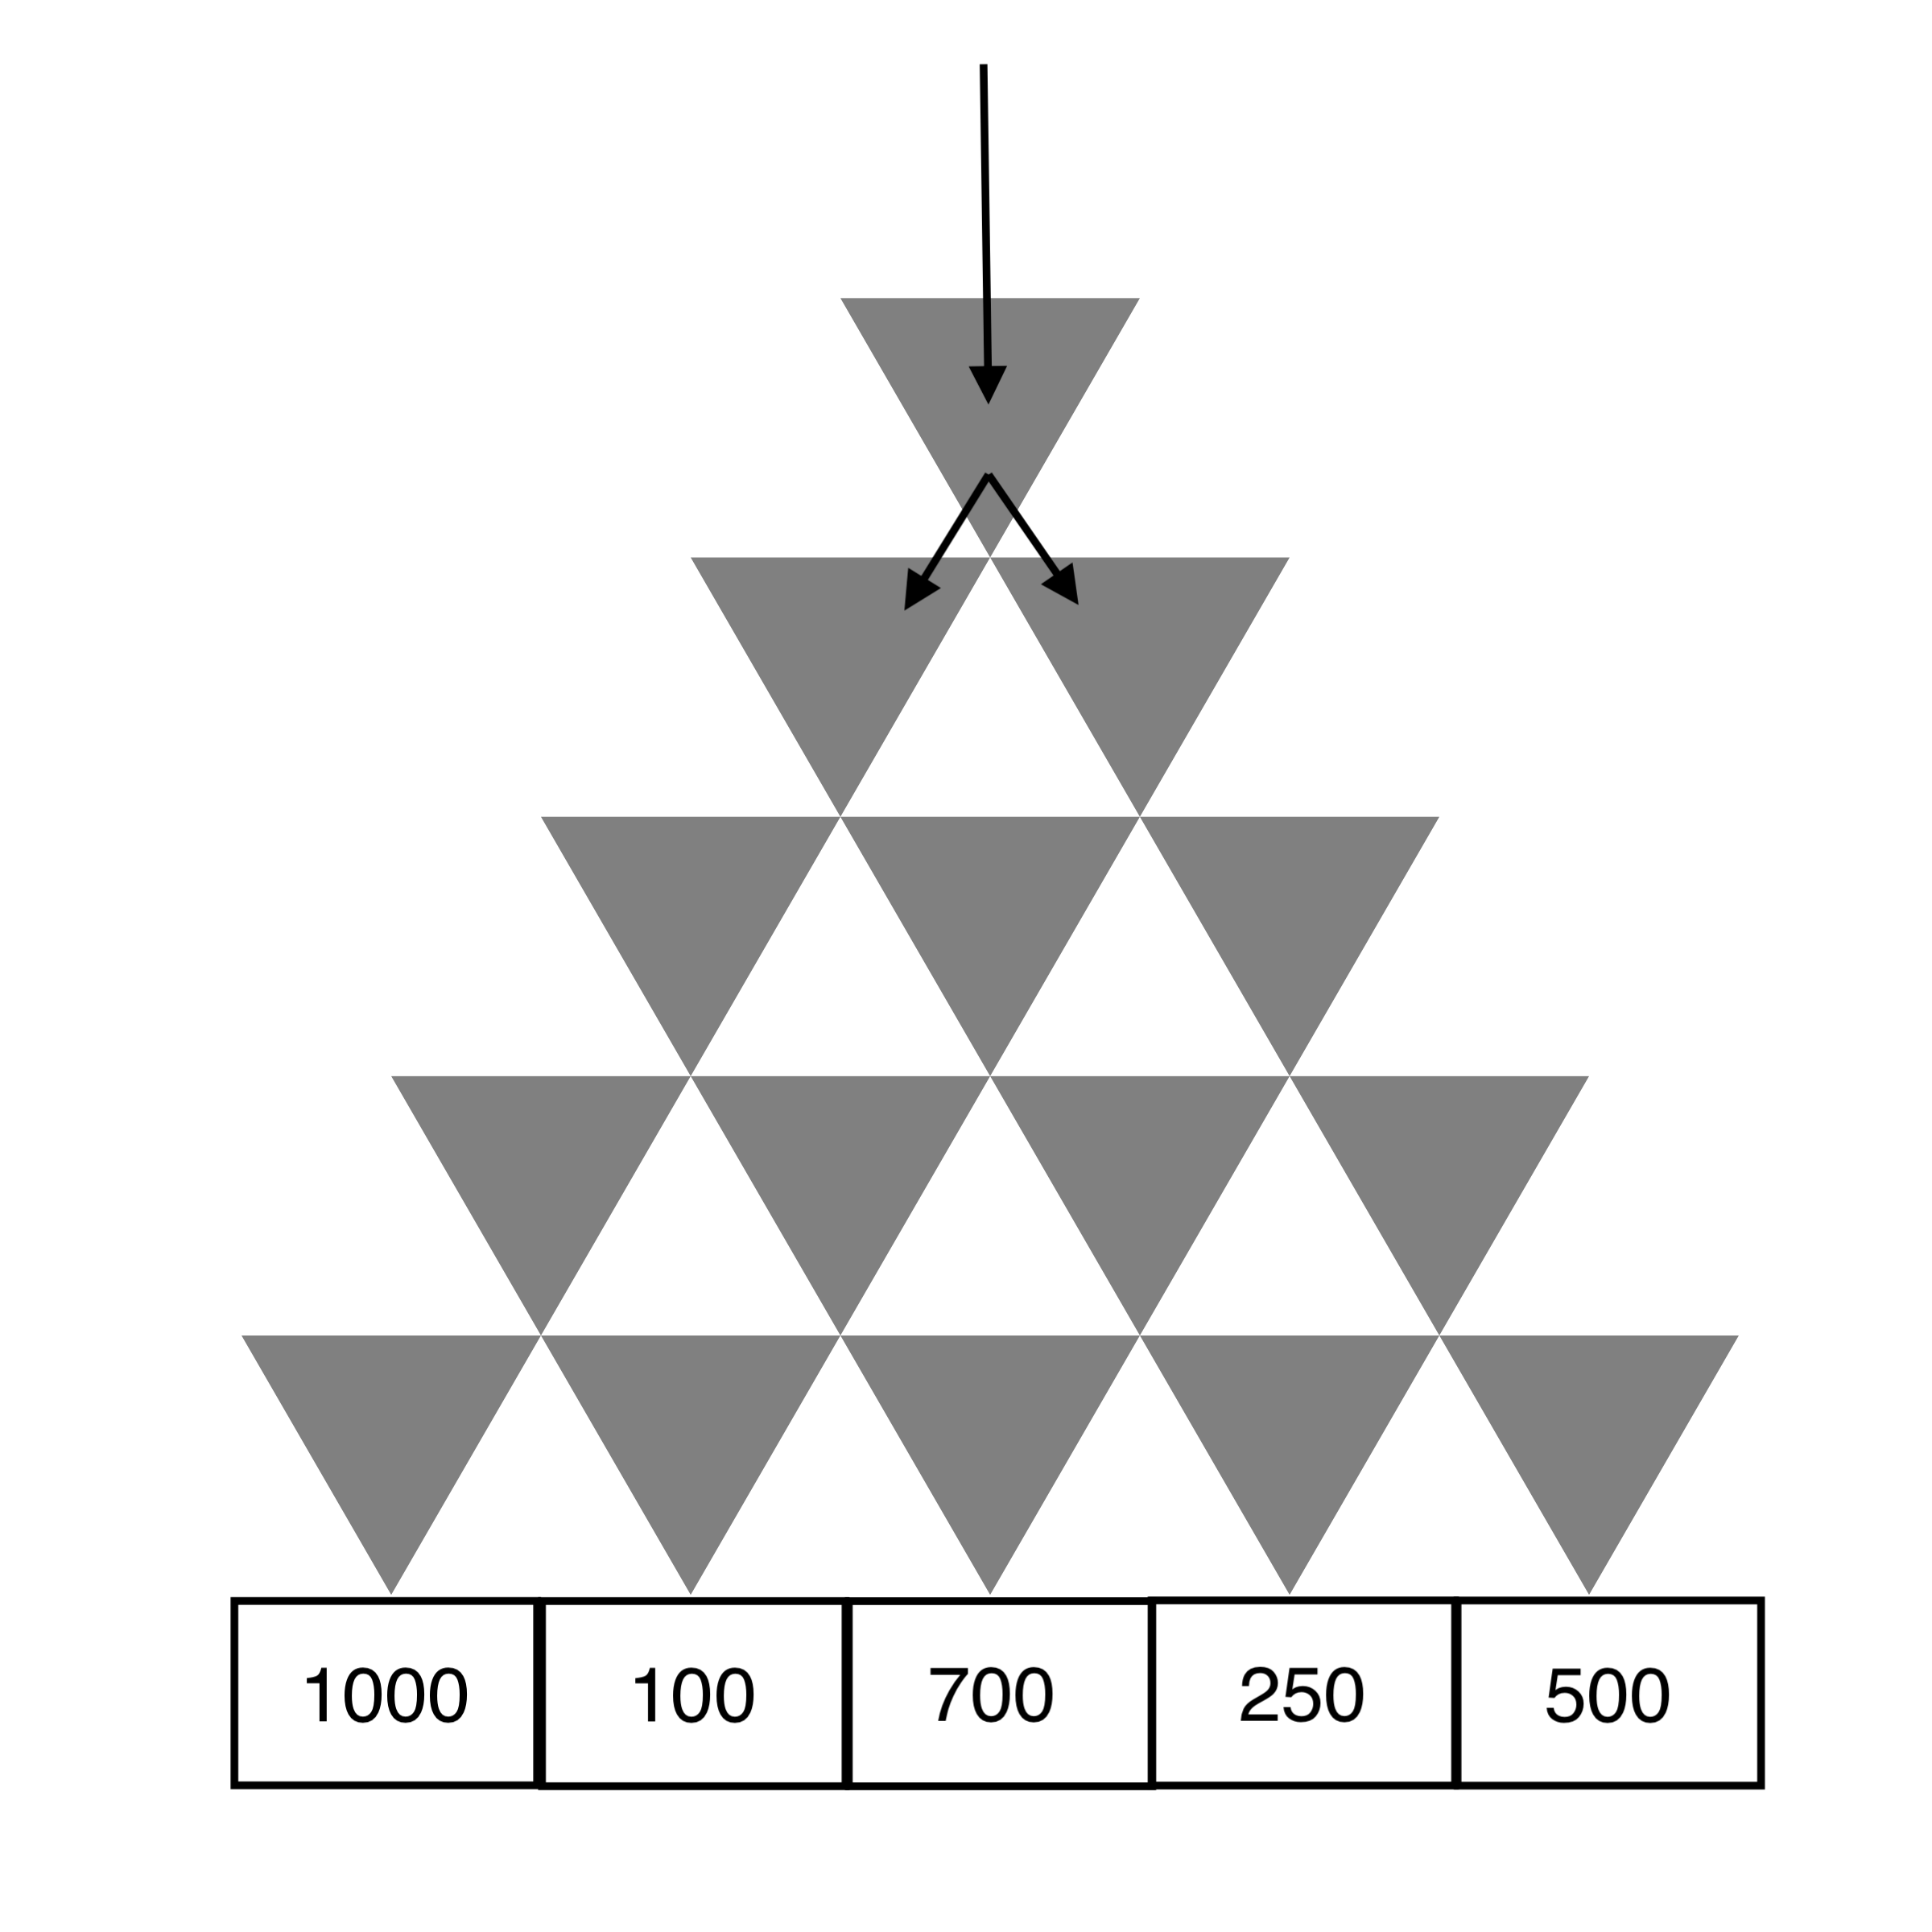
\includegraphics[width=.4\textwidth]{tex/assets/prob-stat/triangles.png}\end{center}
\begin{enumerate}
\item Find the distribution and expected payout for one drop.
\item If balls may be dropped until one reaches the 1000-lev prize, what are the expected number of balls and expected total payout?
\item The host offers to permute the prizes randomly. Would you accept or retain the initial arrangement? How would you arrange the prizes if given the choice?
\end{enumerate}
You suspect that left and right are not equally likely. Let $p$ be the probability of going left.
\begin{enumerate}\setcounter{enumi}{3}
\item Three balls all reach the 100-lev prize. Which $p$ makes this most likely?
\item The show has two pyramids, one with $p=1/2$ and one with $p=1/3$, initially equally likely to be in use. Two balls both reach the middle (700 leva). What is the posterior probability that $p=1/3$?
\end{enumerate}
\end{problempencil}
\begin{problempencil}
One box contains 4 white and 6 black balls; another contains 7 white and 3 black. Draw one random ball from each box, add one white ball, and place these three balls in a third box.
\begin{enumerate}
\item What is the probability that a random ball drawn from the third box is white?
\item Draw from the third box with replacement until the first white ball. For the number $X$ of draws, find $\E X$. Do you think $X$ is geometrically distributed?
\end{enumerate}
\end{problempencil}
\begin{problempencil}[T1, SE 2023]
\begin{enumerate}
\item Let $X\sim Ge(p)$, with $\P(X=k)=pq^k$ for $k\ge0$. Prove the memoryless property: for all $m,n\ge0$, $\P(X>m+n\mid X\ge n)=\P(X>m)$.
\item Prove the converse: if $Y$ takes values in $\{0,1,2,\dots\}$ and $\P(Y>m+n\mid Y\ge n)=\P(Y>m)$ for all $m,n\ge0$, then $Y\sim Ge(p)$ for some $p\ge0$.
\item Let $X_1,\dots,X_n$ be independent, with $X_{\min}:=\min\{X_1,\dots,X_n\}$ and $X_{\max}$ defined similarly. Which of
\[\begin{gathered}
\P(X_1>m)^n,\quad\P(X_1\le m)^n,\quad\P(X_1\le m),\\
1-m\P(X_1>m)^n,\quad1-\P(X_1>m)^n,\quad(1-m)(1-\P(X_1>m)^n)
\end{gathered}\]
represent $\P(X_{\min}\le m)$ and $\P(X_{\max}\le m)$, respectively? Prove your answer.
\item (0.25 points) Roll five standard dice simultaneously. Remove every die showing six, and repeat with the remaining dice until none remain. If $K$ is the total number of rounds, find $\P(K\le n)$ and $\P(K=n)$.
\end{enumerate}
\end{problempencil}
\begin{problempencil}[T1, SE 2023]
Genetic algorithms are heuristics that begin with a ``population'' of chromosomes encoding candidate solutions and evolve towards better solutions. Suppose $n$ chromosomes (Boolean vectors) of length $m$ are initialised with independent $Ber(1/2)$ genes (bits).
\begin{enumerate}
\item What is the probability that all vectors are distinct? What is the expected total number of ones? What is the expected number of vectors containing fewer than $m/4$ zeros?
\item What is the expected number of repetitions, meaning pairs of identical vectors? Answer also for independent $Ber(p)$ bits, $p\in(0,1)$. Which $p$ minimises the expected number of repetitions?
\item \textit{*Bonus: What is the expected number of distinct vectors?}
\item \textit{**Bonus: For fixed $m$, what is the order of magnitude of the smallest $n$ for which the probability that all chromosomes are distinct falls below 50\%?}
\end{enumerate}
\end{problempencil}
\begin{problempencil}[T1, SE 2023]
A television lottery game uses uniformly generated integers from 1 to 5. The rules are:\footnote{\url{https://shorturl.at/bjlqU}}
\begin{itemize}
\item An initial number is drawn (2 in the example).
\item The contestant may stop and take the prize below the latest number, or guess whether the next number will be smaller or larger. \textbf{Consecutive numbers are guaranteed to differ.}
\item A wrong guess ends the game with no prize. After a correct guess the contestant may continue, up to the grand prize of 1000 leva.
\end{itemize}
\begin{center}\begin{tabular}{cccc}2&$\longrightarrow ?$&$\longrightarrow ?$&$\longrightarrow ?$\\0 leva&10 leva&100 leva&1000 leva\end{tabular}\end{center}
\begin{enumerate}
\item Propose a strategy, compute its win probability and expected payout if the contestant commits to exactly $k$ guesses, $k=0,1,2,3$. Compare it with choosing smaller/larger independently with probability $1/2$ each time.
\item \textit{Bonus: Write pseudocode for numbers from $0$ to $n$, $m$ guesses and prizes $c_0,\dots,c_n$.}
\item \textit{Bonus: Write pseudocode determining whether stopping or guessing again is optimal after each round of the general game in part 2.}
\end{enumerate}
\end{problempencil}
\begin{problempencil}
Angel is a young Pok\'emon trainer. Ten flying species live near his town, and he estimates that encountering a Pok\'emon takes half an hour.
\begin{enumerate}
\item Assuming all ten species are equally rare, how long does he expect to need to encounter all of them?
\item Let $X_i$ be the number of encounters up to the first of species $i$. Find its distribution and express the quantity in part 1 using the $X_i$.
\item Inclusion--exclusion also works for maxima and minima; for example, $\max\{x_1,x_2\}=x_1+x_2-\min\{x_1,x_2\}$. Generalise to $n$ numbers.
\item If $Y_1,Y_2$ are independent geometric variables with parameters $p_1,p_2$, find the distribution of $\min\{Y_1,Y_2\}$.
\item Angel realises that equal rarity is unrealistic. Answer part 1 when the probability of species $i$ is proportional to $i$. \textit{For an explicit answer, use four species.}
\end{enumerate}
\end{problempencil}
\begin{problempencil}[E, SE 2024]
Box A contains slips numbered 1 through 10. Angel chooses $K$ uniformly from 1 through 10 and transfers $K$ randomly selected slips from A to B.
\begin{enumerate}
\item What is the expected number on a randomly drawn slip from B?
\item What is the probability that B contains two numbers summing to 11?
\item Let $X$ be the smallest number in B and $N$ the number of draws with replacement from B until $X$ first appears. Is $N$ geometric, and if so with what parameter? Find $\E[N]$.
\end{enumerate}
\end{problempencil}
\begin{problempencil}[T1, AM/Mathematics 2024]
Let $n$ be positive. Choose $u_1$ uniformly among the integers in $[1,n]$, then $u_2$ from $[1,u_1-1]$, $u_3$ from $[1,u_2-1]$, and so on until $u_\ell=1$, $\ell\le n$. Let $E_n:=\{u_1,\dots,u_\ell\}$.
\begin{enumerate}
\item Find $\P(k\in E_n)$ for $k\le n$.
\item Find $\P(2\in E_n\mid3\notin E_n)$.
\item Find $\Ebb{|E_n|}$ and $D(|E_n|)$ and estimate their asymptotic behaviour as $n\to\infty$.
\end{enumerate}
\end{problempencil}
\begin{problempencil}[T1, AM/Mathematics 2024]
\begin{enumerate}
\item Let $X$ be random in $\{0,1,2\}$ and $Y\sim Ber(2/3)$ independent of it. Find the joint distribution and correlation of $X$ and $Z:=(X+Y)\pmod3$.
\item Let $X$ be uniform on $\{1,\dots,6\}$. Find its probability generating function and express $\Ebb X$ and $DX$ in terms of it.
\item (0.5 points) For nonnegative integer-valued $X,Y$, does independence imply $g_X(s)g_Y(s)=g_{X+Y}(s)$ for every $s\ge0$? Does that identity for every $s\ge0$ imply independence? Prove your assertions.
\item Let $X,Y$ be the results of two independent standard dice. Find the law of $X+Y$. Can two blank six-sided dice be labelled with different positive integers, not necessarily identically on the two dice, so that their sum has the same distribution as $X+Y$?
\end{enumerate}
\end{problempencil}
\pagebreak
\noindent Summer semester, 2024/2025\hfill 4. Geometric probability
\par\noindent\hrulefill\par
\begin{problembook}
A point A is chosen randomly on a diameter of a circle of radius $R$. A chord through A is drawn perpendicular to the diameter. What is the probability that the chord is shorter than $R$?
\end{problembook}
\begin{problembook}
Two ships must unload at the same berth on the same day. Their arrival times are independent and may be anywhere within the 24-hour day. What is the probability that they do not overlap if unloading takes 6 hours for the first and 4 for the second?
\end{problembook}
\begin{problem}
Buses on route A run every five minutes and those on route B every ten minutes, independently of route A. What is the probability that
\begin{enumerate}\item an A bus arrives before a B bus;\item a passenger arriving at a random time waits at most two minutes?\end{enumerate}
\end{problem}
\begin{problembook}
A segment has length $K$. Two other segments with lengths less than $K$ are chosen randomly. What is the probability that the three can form a triangle?
\end{problembook}
\begin{problembook}
What is the probability that three randomly chosen segments, each shorter than $K$, can form a triangle?
\end{problembook}
\begin{problem}
A recording tape is 100 m long. A continuous 20 m message is recorded at a random location on each side. What is the probability that every point between 25 m and 50 m from the beginning contains at least one of the messages?
\end{problem}
\begin{problembook}
Numbers $x,y$ are independently and uniformly chosen in $(0,1]$. Find the probabilities of
\begin{enumerate}
\item $xy\le1/4$;
\item $x+y\le1$ and $x^2+y^2\ge1/2$;
\item $xy\ge2/5$ and $x^2+y^2\le1$.
\end{enumerate}
\end{problembook}
\begin{problembook}A unit segment is randomly divided into three parts. What is the probability that they form a triangle?\end{problembook}
\begin{probleminteresting}[Bertrand's paradox]
An equilateral triangle is inscribed in a circle of radius 1. What is the probability that a randomly selected chord is longer than a side of the triangle?
\end{probleminteresting}
\pagebreak
\noindent Summer semester, 2024/2025\hfill 5. Continuous distributions
\par\noindent\hrulefill\par
\begin{problembook}
A random variable $X$ has density $f_X(x)=\begin{cases}c(x^2+2x),&x\in[0,1],\\0,&x\notin[0,1].\end{cases}$ Find
\begin{enumerate}\item $c$;\item $\E X$ and $DX$;\item the probability that $X$ is smaller than its expectation;\item the expectation of $X^2+3X$.\end{enumerate}
\end{problembook}
\begin{problembook}
A is fixed on a circle $k(O,r)$, and B is chosen randomly on the circumference. Find the expected area of $\triangle AOB$.
\end{problembook}
\begin{problembook}
A device's lifetime in years is $X\sim U(0,7)$. Under its warranty it is replaced after five years, or sooner if it fails. Let $Y$ be the time until replacement. Compute $\P(Y<4)$, $\E Y$ and $DY$. If 1000 devices are sold, how many are expected to need replacement before year five?
\end{problembook}
\begin{problem}
Points A and B are chosen randomly inside a disk of radius $R$. Find the probability that the circle centred at A with radius AB lies inside the disk.
\end{problem}
\begin{problembook}
Two cashiers have exponential customer service times with means 8 and 5 minutes, respectively. A customer chooses a queue randomly and waits less than four minutes. What is the probability that this was the first queue?
\end{problembook}
\begin{problembook}
A medical examination has an exponential duration with mean 30 minutes. Two patients have appointments at 11:00 and 11:30 and both arrive punctually. The second waits if the first examination has not finished. Find the expected total time the second patient spends at the clinic.
\end{problembook}
\begin{problembook}
For $X\sim Exp(\lambda)$, find the densities of
\begin{itemize}\item $Y=-X$;\item $Y=2X-1$;\item $Y=\sqrt X$;\item $Y=X^\alpha$, $\alpha>0$.\end{itemize}
\end{problembook}

\begin{problem}
A light ray travels from $(0,2)$ to $(0,1)$, where it is refracted at a random angle $\theta\in(-\pi/2,\pi/2)$ to the $y$-axis. Let $X$ be the point where the refracted ray meets the $x$-axis. Find the density of $X$.
\end{problem}
\begin{problembook}
A coin with heads probability $3/4$ is tossed 2000 times. What is the probability that the number of heads lies between 1475 and 1535?
\end{problembook}
\begin{problem}
A point $(X,Y)$ is chosen uniformly in the triangle with vertices $(0,0)$, $(0,2)$ and $(3,0)$. Find the joint density, distribution function and correlation of $X,Y$.
\end{problem}
\begin{problembook}
An anti-burglary device switches house lights on at time $X$ and off at time $Y$ during a fixed hour. Their joint density is $f_{X,Y}(x,y)=cxy$ for $0<x<y<1$. Find
\begin{enumerate}
\item $c$;
\item the marginal densities and expectations;
\item the probability that the lights turn on before minute 45 and remain on for less than 10 minutes;
\item the expected duration if they turn on at minute 15;
\item the probability that they remain on for less than 20 minutes.
\end{enumerate}
\end{problembook}
\begin{problem}
Two points are chosen independently and randomly on the boundary of a square of side $a$. Find the expected squared distance between them.
\end{problem}
\begin{problembook}
For independent $X_1,X_2\sim Exp(\lambda)$, find the distribution of $Y=X_1/(X_1+X_2)$.
\end{problembook}
\begin{problembook}
For independent $X_1,X_2\sim U(0,1)$, find the distribution of $Y=X_1+X_2$.
\end{problembook}
\begin{problembook}
For independent $X_1,X_2\sim Exp(\lambda)$, find the density of
\begin{enumerate}\item $Y=\max(X_1,X_2)$;\item $Y=\min(X_1,X_2)$.\end{enumerate}
\end{problembook}
\begin{problem}
A point $P$ is chosen randomly inside a triangle of area 1. The line through $P$ parallel to one side meets the other sides at $Q,R$. Points $S,T$ lie on the base so that $QRST$ is a rectangle. Find $\E S_{QRST}$.
\end{problem}
\begin{problempencil}
Two instruments measure airborne dust. If the true concentration is $x\,\mathrm{g/m^3}$, the first reading is normal with mean $x$ and standard deviation $0.05x$, and the second is normal with mean $x$ and standard deviation $0.1x$. Which would you use? For each, what is the probability of an error exceeding $0.1x$? If independent readings are averaged, what is the probability that the average has error exceeding $0.1x$?
\end{problempencil}
\begin{problempencil}
Let $\xi\sim Exp(2)$ and $\eta\sim U(0,3)$ be independent, with
\[f_\xi(x)=\begin{cases}2e^{-2x},&x>0,\\0,&\text{otherwise},\end{cases}\qquad
f_\eta(x)=\begin{cases}1/3,&0<x<3,\\0,&\text{otherwise}.\end{cases}\]
Find their correlation, $\P(\xi<\eta)$ and the density of $\xi/\eta$.
\end{problempencil}
\begin{problempencil}[T2, SE 2020]
A point A is chosen randomly in the unit disk centred at O. Let $X=|OA|$. Guess its mode and median and justify your guesses. What do you expect $\E X$ to be? \textit{A discrete mode is a value with greatest probability; for a density, a mode maximises $f_X$. Here $a$ is a median if $\P(X\le a)=\P(X\ge a)=1/2$.}
\begin{enumerate}
\item Find the distribution function, density, expectation and variance of $X$.
\item Choose three independent random points $A_1,A_2,A_3$ in the same disk. Find the expected distance to the nearest point and to the farthest point. \textit{Bonus: find the expected distance to the middle point. Should it equal $\E X$?}
\end{enumerate}
\end{problempencil}
\begin{problempencil}[T2, Probability and Statistics 2021]
Information boards at bus stops contain $10\times100$ LEDs. Each LED's lifetime is modelled as exponential with mean ten years. A board needs repair when fewer than 75\% of its LEDs work, making it hard to read. What is the probability of requiring repair after three years?
\end{problempencil}
\begin{problempencil}[T2, Probability and Statistics 2021]
The returns of assets A, B and C are independent normal variables $N(3,2)$, $N(3,3)$ and $N(1,10)$. You have five units to invest.
\begin{enumerate}
\item How should you allocate them to maximise expected profit?
\item Among the allocations in part 1, which minimises variance?
\item A risk-taking investor puts all five units into an independent asset $D\sim N(-2,20)$. What is the probability that this investment outperforms the one in part 2?
\end{enumerate}
\end{problempencil}
\begin{problempencil}[T2, Probability and Statistics 2021]
X and Y travel together from town A to B, then wait for buses to C and D, respectively. Travel times are $T_{AB}\sim Exp(3)$, $T_{BC}\sim Exp(4)$ and $T_{BD}\sim Exp(5)$; waiting times in B are $T_C\sim Exp(1)$ and $T_D\sim Exp(2)$. All these times are independent. Let $\xi,\eta$ be the total journey times of X and Y.
\begin{center}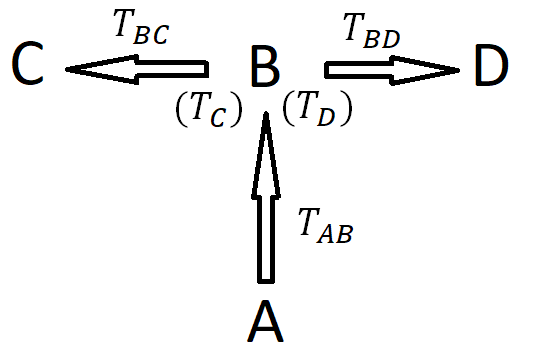
\includegraphics[width=7cm]{tex/assets/prob-stat/buses2.png}\end{center}
\begin{enumerate}\item Find $\P(T_C+\ln(\E T_D)>0)$.\item Find $Cor(\xi,\eta)$.\end{enumerate}
\end{problempencil}
\begin{problempencil}[E, Probability and Statistics / SE 2021]
A and B generate independent $U([0,1])$ numbers in rounds, one each per round. They want to estimate how often a number exceeds 0.75 and consider two procedures:
\begin{enumerate}
\item Each generates five numbers, and they compute the proportion above 0.75 among all ten.
\item Each generates 500 numbers instead. Find the mean and variance of the estimate under each procedure. Which would you choose, and why?
\item Over many rounds, what fraction have both numbers above 0.75? What is the expected number of rounds until at least one number exceeds 0.75?
\end{enumerate}
\begin{it}Example:
\begin{center}\begin{tabular}{l|ccccc}Round&1&2&3&4&5\\\hline
A&0.167&0.518&0.991&0.364&0.496\\
B&0.296&0.840&0.755&0.143&0.646
\end{tabular}\end{center}
Here the proportion in part 1 is $3/10$, the proportion in part 3 is $1/5$, and the first round with at least one number above 0.75 is round 2.
\end{it}
\end{problempencil}
\begin{problempencil}[T2, Probability and Statistics 2022]
Insurer ``Ins 1'' models claim sizes as independent exponential variables with mean 100 leva. It pays $x>0$ leva to ``Ins 2'' for reinsurance: whenever a claim exceeds 300 leva, Ins 2 covers 200 leva.
\begin{enumerate}
\item (0.25 points) What is the probability that Ins 1 pays less than 200 leva from its own budget for one claim?
\item (0.25 points) If Ins 2 requires an expected profit of 10 leva per claim, what should $x$ be?
\item (0.5 points) What policy price gives Ins 1 an expected profit of 10 leva per claim? What would the price be without reinsurance? Why might Ins 1 want reinsurance when expected profit is the same?
\end{enumerate}
\end{problempencil}
\begin{problempencil}
Let $(X_j)_{j\ge1}$ be independent $Exp(1)$ variables and $M_n=\max\{X_1,\dots,X_n\}$.
\begin{enumerate}
\item (0.25 points) Find the distribution functions of $M_2$ and $M_n$.
\item (0.75 points) Show that $Y_n=M_n-\log n$ converges in distribution to a variable $Y$, and find its distribution function.
\end{enumerate}
\end{problempencil}
\begin{problempencil}
Without internet access, a computer user estimates $\pi$ by simulating many uniform points in $[0,1]\times[0,1]$ and measuring the fraction inside its inscribed circle. Explain how and why this estimates $\pi$. How many points are needed for an error smaller than 0.001 with probability 95\%?
\end{problempencil}
\begin{problempencil}
The historical mean January temperature in Sofia is given as $-0.5^\circ\mathrm C$. Let $X$ be the mean January temperature and assume a normal distribution. Variance is normally estimated from data; here consider a different, unrecommended approach. Suppose temperatures above $20^\circ\mathrm C$ are considered extreme, with probability 1\%. What variance estimate does this imply? What would be the probability of a temperature below $-15^\circ\mathrm C$?
\end{problempencil}
\begin{problempencil}
The mass of peas in a can is modelled as $N(\mu,10^2)$ grams, and 15\% of cans contain less than 250 grams. Find
\begin{enumerate}
\item (0.25 points) $\mu$;
\item (0.25 points) the percentage containing more than 280 grams.
\end{enumerate}
After a change, the model is $N(250,\sigma^2)$.
\begin{enumerate}\setcounter{enumi}{2}\item (0.5 points) Find $\sigma$ if 97\% contain between 230 and 270 grams.\end{enumerate}
\end{problempencil}
\begin{problempencil}
A random byte represents an integer from $00000000_{(2)}$ to $11111111_{(2)}$, i.e. from $0_{(10)}$ to $255_{(10)}$. From left to right, the first bit is 1 with probability $1/2$, the second with probability $1/4$, and so on.
\begin{center}\begin{tabular}{|c|c|c|c|c|c|c|c|}\hline0&1&0&0&0&1&1&1\\\hline\end{tabular}\end{center}
\begin{enumerate}\item What is the expected number of ones?\item What is the expected decimal value of the byte? The example above represents 71.\end{enumerate}
\end{problempencil}
\begin{problempencil}
A property near FMI costs EUR 250,000. An experienced agent negotiates a percentage price change $X_1\sim N(-10,10)$. Negotiating yourself produces a percentage change $X_2\sim N(0,100)$, independent of $X_1$.
\begin{enumerate}
\item What is the probability of obtaining a better price by negotiating yourself?
\item What is the probability of a price below EUR 225,000 in each case?
\end{enumerate}
\end{problempencil}
\begin{problempencil}[T1, SE 2022]
Choose X randomly on a unit segment OA, then Y randomly on XA. What is the probability that OX, XY and YA form a triangle?
\end{problempencil}
\begin{problempencil}[T2, SE 2022]
A point starts at the origin. At each step it chooses uniformly among the four axis directions and moves one unit. An example ten-step path is shown below.
\begin{center}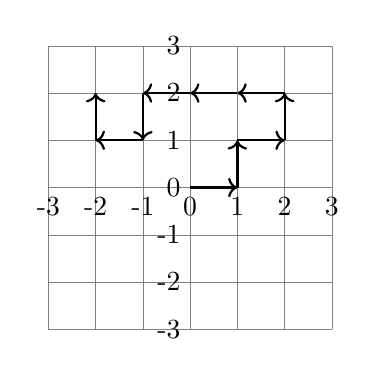
\begin{tikzpicture}[scale=.6]
\draw[step=1cm,gray,very thin](-3,-3)grid(3,3);
\foreach \x in {-3,-2,...,3}{\node[anchor=north]at(\x,0){\x};}
\foreach \y in {-3,-2,...,3}{\node[anchor=east]at(0,\y){\y};}
\draw[->,thick](0,0)--(1,0);\draw[->,thick](1,0)--(1,1);\draw[->,thick](1,1)--(2,1);\draw[->,thick](2,1)--(2,2);\draw[->,thick](2,2)--(1,2);\draw[->,thick](1,2)--(0,2);\draw[->,thick](0,2)--(-1,2);\draw[->,thick](-1,2)--(-1,1);\draw[->,thick](-1,1)--(-2,1);\draw[->,thick](-2,1)--(-2,2);
\end{tikzpicture}\end{center}
\begin{enumerate}
\item What is the probability that its $x$-coordinate exceeds 10 after 1000 steps?
\item Find the expectation and variance of the squared distance from the origin after 100 steps.
\end{enumerate}
\end{problempencil}
\begin{problempencil}[T2, SE 2022]
Let $X_0\sim Exp(1)$ and $X_n=2X_{n-1}+\epsilon_n$ for $n\in\N$, where the $\epsilon_n$ are independent $N(0,1)$ variables.
\begin{enumerate}
\item Find $\E X_n$ and $DX_n$.
\item For $S_{n,1}=\sum_{i=1}^n(X_n-2X_{n-1})^2$ and $S_{n,2}=\sum_{i=1}^n|X_n-2X_{n-1}|$, find $\E S_{n,1}$ and $\E S_{n,2}$.
\item Answer parts 1 and 2 when $\epsilon_i\sim N(1,2)$.
\end{enumerate}
\end{problempencil}
\begin{problempencil}[E, SE 2022]
Each cell of a $9\times9$ grid is coloured randomly white, green or red.
\begin{center}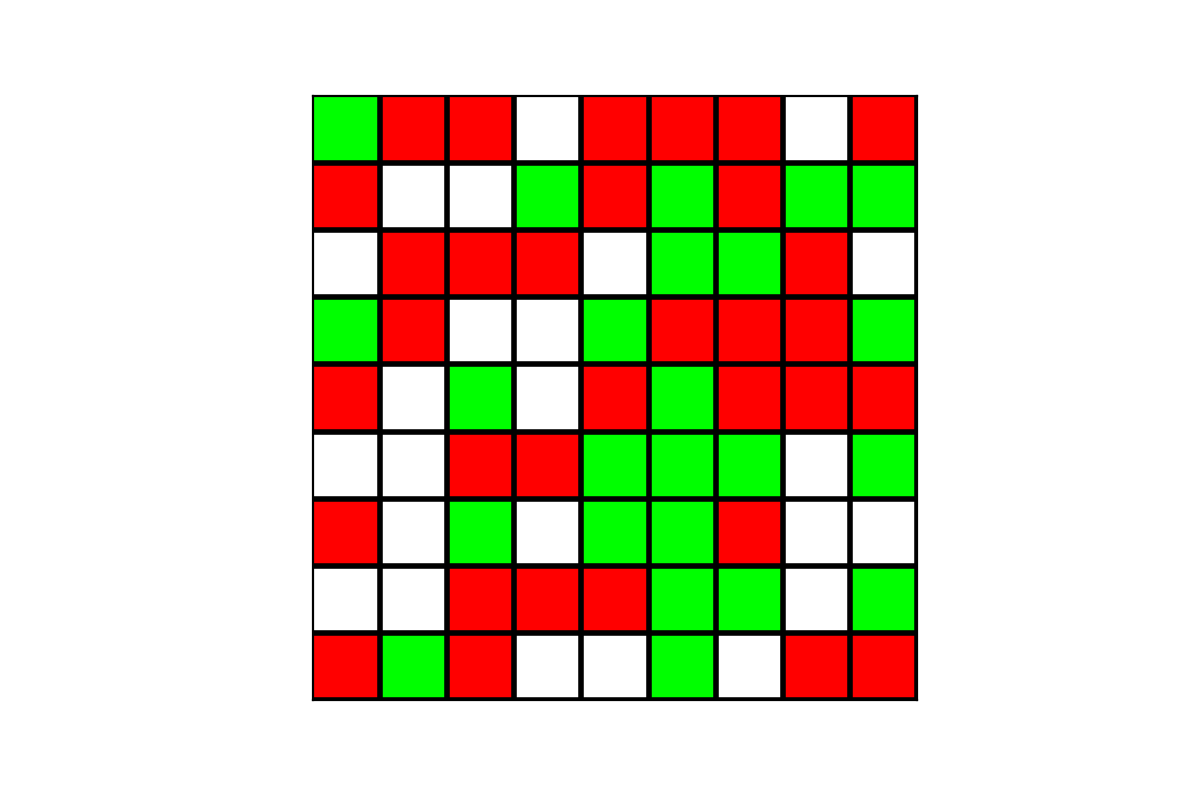
\includegraphics[width=.5\textwidth]{tex/assets/prob-stat/grid.png}\end{center}
\begin{enumerate}
\item What is the expected number of white or green cells? What is the probability of at least 60? A horizontal (vertical) flag consists of three consecutive horizontal (vertical) cells coloured white, green, red from left to right (top to bottom).
\item Is the number of horizontal flags binomial, and if so with what parameters?
\item What is the expected number of horizontal flags?
\item Are the numbers of horizontal and vertical flags independent? What is their expected total number?
\end{enumerate}
\end{problempencil}
\begin{problempencil}[E, SE 2022]
Let $X_1,X_2,\dots$ be independent $Exp(1)$ variables and $S_n=X_1+\cdots+X_n$.
\begin{enumerate}
\item Find the density of $S_2$ and prove by induction that
\[f_{S_n}(x)=\frac{x^{n-1}}{(n-1)!}e^{-x}\one_{\{x>0\}}.\]
\item Let $N_t:=\max\{n:S_n\le t\}$. Prove $\P(N_t\ge n)=\P(S_n\le t)$ and $\P(N_t=n)=\P(S_n\le t)-\P(S_{n+1}\le t)$.
\item Find the distribution of $N_t$.
\end{enumerate}
\end{problempencil}
\begin{problempencil}[E, Probability and Statistics 2023]
Let $U\sim U(0,1)$ and $V\sim U(-\pi/2,\pi/2)$.
\begin{enumerate}
\item One way to generate a pseudorandom number from $U$ is to choose a usually large positive integer $M$ and use the fractional part $X:=\{MU\}$. Find $\E X$, $DX$ and $Cor(U,X)$. What do you think of this method?
\item For iid $U_1,\dots,U_{100}\sim U$, find the expectation of each and of their maximum and minimum.
\item Find the density, expectation and variance of $Y:=\tan V$.
\item Let $Z\sim Cauchy(1)$, with $f_Z(x)=1/(\pi(1+x^2))$, $x\in\R$. Prove that $1/Z$, $2Z/(1-Z^2)$ and $(3Z-Z^3)/(1-3Z^2)$ have the same distribution.
\end{enumerate}
\end{problempencil}
\begin{problemstarpencil}[E, Probability and Statistics 2023]
\begin{enumerate}
\item (0.25 points) Define $D(Y\mid X):=\E((Y-\E(Y\mid X))^2\mid X)$. Recall $\E X=\E(\E(X\mid Y))$. Which of the following expresses $DY$?
\[\begin{gathered}\E(D(Y\mid X)),\quad D(D(Y\mid X)),\\\E(D(Y\mid X))+D(D(Y\mid X)),\quad\E(D(Y\mid X))+D(\E(Y\mid X)).\end{gathered}\]
\end{enumerate}
Construct the Cantor function $c:[0,1]\to[0,1]$ recursively: $c(x)=1/2$ on $[1/3,2/3]$, $c(x)=c(3x)/2$ on $[0,1/3)$ and $c(x)=(1+c(3x-2))/2$ on $(2/3,1]$.
\begin{figure}[ht]\centering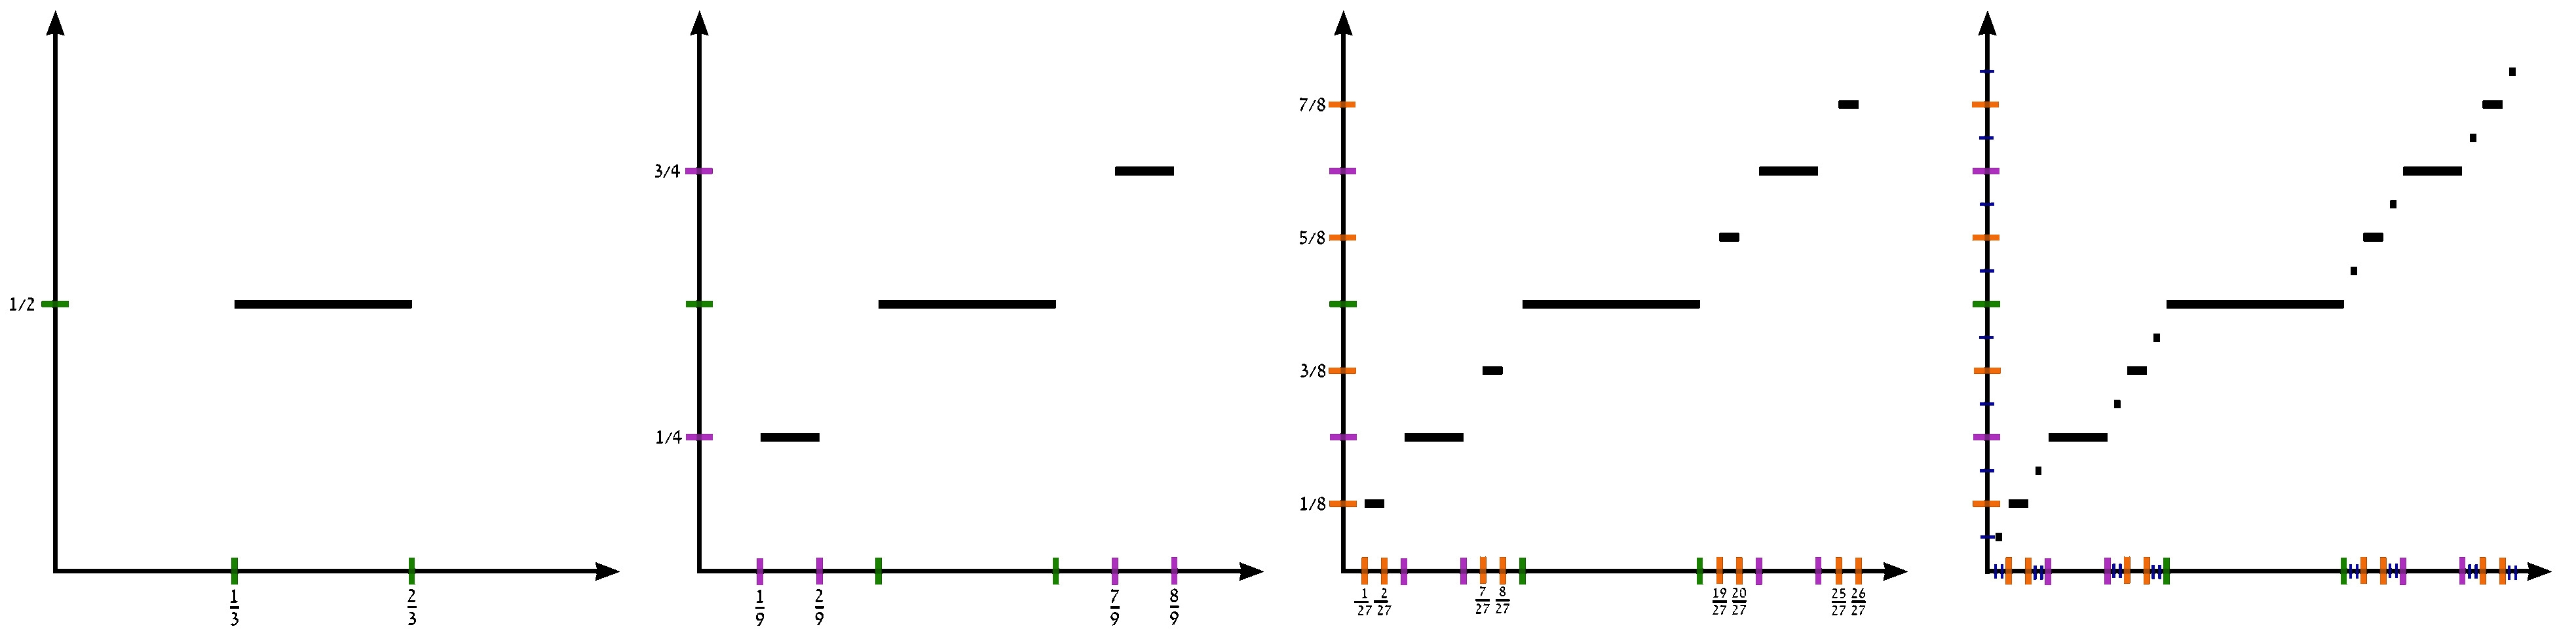
\includegraphics[width=\textwidth]{tex/assets/prob-stat/Cantor.jpg}\caption{Recursive construction of the Cantor function. Source: \href{https://en.wikipedia.org/wiki/Cantor_function}{Wikipedia}.}\end{figure}
\begin{enumerate}\setcounter{enumi}{1}
\item Let $X$ have $F_X(x)=c(x)$ on $(0,1)$. Find $\E X$ and $DX$.
\item Prove that $F_X$ is differentiable almost everywhere. What is its density $f_X$?

\end{enumerate}
\end{problemstarpencil}
\begin{problempencil}[E, Probability and Statistics / SE 2023]
The joint density is $f_{X,Y}(x,y)=cx+y$ for $x,y\ge0$, $x+2y\le1$, and zero elsewhere.
\begin{enumerate}
\item Find $c$, the density of $X$, and $\E Y$.
\item Find $\E(Y\mid X=1/2)$.
\item Find the densities of $Z=X+2Y$ and of $Z=XY$.
\item Let $(X_1,Y_1),\dots,(X_n,Y_n)$ be iid copies of $(X,Y)$. For large $n$, estimate $\P(X_1+\cdots+X_n>Y_1+\cdots+Y_n)$.
\end{enumerate}
\end{problempencil}
\begin{problempencil}[T2, Probability and Statistics 2023]
Benford's law,\footnote{The source attributes the observation to Newcomb's logarithm tables in 1881 and to Benford's larger dataset in 1934.} also called the first-digit law, is the empirical observation that the leading nonzero digit in many real datasets is not uniform, and is most often 1 (in bases other than ten as well). The decimal Benford distribution assigns probability $\log_{10}(1+1/d)$ to $d\in\{1,\dots,9\}$. To accuracy 0.01, find the probability that the leading nonzero decimal digit of $X$ is 1 when
\begin{enumerate}
\item $X\sim N(0,1)$;
\item $X\sim Exp(1)$;
\item $X=U_1/U_2$ for independent $U_1,U_2\sim U(0,1)$. Find $\E X$.
\item \textit{Bonus: $X$ is a ``random positive power of 2''. More precisely, find $\lim_{n\to\infty}\P(X_n\text{ starts with 1})$, where $X_n=2^{U_n}$ and $U_n\sim U(\{1,2,\dots,n\})$.}
\end{enumerate}
Compare with Benford's distribution.\footnote{If time permits, compute the probabilities for other leading digits too and compare with Benford's distribution.}
\end{problempencil}
\begin{problempencil}[T2, Probability and Statistics 2023]
Let $X_1,X_2\sim\Gamma(3,2)$, with density $f_X(x)=4x^2e^{-2x}\one_{\{x>0\}}$.
\begin{enumerate}
\item Find the density of $Y=X_1/(X_1+X_2)$.
\item Find $Cor(X_1,X_2)$ and $Cor(X_1+X_2,Y)$.
\item Are $X_1+X_2$ and $Y$ independent?
\end{enumerate}
\end{problempencil}
\begin{problempencil}[T2, Probability and Statistics 2023]
A chip manufacturer claims that only one in 1000 chips is defective.
\begin{enumerate}
\item How would you use the central limit theorem (CLT) to approximate the probability of at least one defective chip among 100? What alternatives would you suggest?
\item The Berry--Esseen inequality states that for iid variables $X_1,\dots,X_n$ with
\[\mu:=\E X_1,\quad\sigma:=\sqrt{DX_1},\quad\rho:=\Ebb{|X_1-\mu|^3}<\infty,\quad Z_n:=\frac{X_1+\cdots+X_n-n\mu}{\sigma\sqrt n},\]
we have
\[\sup_{x\in\R}|\P(Z_n\le x)-\Phi(x)|\le\frac{\rho}{2\sigma^3\sqrt n}.\]
How can this help in part 1? Assuming the manufacturer's claim is correct, for which $n$ is the CLT approximation error less than 0.001?
\end{enumerate}
\end{problempencil}
\begin{problem}
Let $X,Y$ be independent exponential variables with rates $1/\alpha$ and $1/\beta$, and let $X_1,\dots,X_n$ be independent observations of $X$.
\begin{enumerate}
\item (0.25 points) For $\overline X=(X_1+\cdots+X_n)/n$ and large $n$, find $c$ such that $\P(|\alpha-\overline X|>c)\le1\%$.
\end{enumerate}
Let $Z=\sqrt{X/Y}$ and $Z_1,\dots,Z_n$ be independent observations of $Z$.
\begin{enumerate}\setcounter{enumi}{1}
\item (0.75 points) Is it true that
\[\frac{Z_1+\cdots+Z_n}{n}\xrightarrow[n\to\infty]{\mathrm{a.s.}}\sqrt{\frac{\Ebb X}{\Ebb Y}}\,?\]
Prove it if true; otherwise find the limit.
\end{enumerate}
\end{problem}
\begin{problem}
A die has faces labelled 1, 1, 3, 3, 5, 7. Let $X$ be the result of one roll.
\begin{itemize}
\item (0.25 points) Find its distribution, expectation and variance. What is the probability that exactly four of five rolls are either 3 or 7?
\item (0.25 points) Approximate the probability that the sum of 100 rolls exceeds 2222. What about 4444?
\item (0.25 points) Find the expected number of rolls until the hundredth 7, and the expected number of 3s by that time.
\end{itemize}
\end{problem}
\begin{problempencil}[E, Probability and Statistics / SE 2024]
An FMI student designs a roulette wheel whose past colours influence future outcomes:
\begin{itemize}
\item there are only black and red numbers;
\item on spin $n+1$, the probability of red is $P_n(m):=(1+m)/(2+n)$, where $m$ is the number of red results so far.
\end{itemize}
Let $X_n:=\ind{\{\text{spin }n\text{ is red}\}}$. Given $(X_1,\dots,X_n)$, the conditional law of $X_{n+1}$ is Bernoulli with parameter $P_n(\sum_{i=1}^nX_i)$. For example, red, red, black gives $(X_1,X_2,X_3)=(1,1,0)$ and successive red probabilities $(1/2,2/3,3/4,3/5)$, so $\P(X_4=1\mid X_1=1,X_2=1,X_3=0)=P_3(2)=3/5$.
\begin{enumerate}
\item (0.25 points) Prove that, for any permutation $\sigma$ of $\{1,\dots,n\}$,
\[\P(X_1=x_1,\dots,X_n=x_n)=\P(X_{\sigma(1)}=x_1,\dots,X_{\sigma(n)}=x_n).\]
Thus the vector and every permutation of it have the same law.
\item (0.25 points) Find $\P(X_n=0)$ and $Cov(X_i,X_j)$ for $i\ne j$.
\item (0.25 points) Find the law of the number $W_4$ of red outcomes in four spins, and of $W_n$ in $n$ spins.
\item (0.25 points) Find $\P(X_m=0\mid X_n=1)$ for every $m,n$.
\item (0.25 points) Find the probability that spins $n$ and $n+1$ have the same colour.
\item (0.25 points) Compute $\P(W_{n+1}=W_n+1)$.
\item \textit{Bonus* (0.5 points): Prove that $P_n$ converges in distribution and find its limit.}
\item \textit{Bonus* (0.25 points): Give an algorithm constructing a roulette wheel numbered 1 through 36, with even numbers red, that realises these probabilities.}
\end{enumerate}
\end{problempencil}
\begin{problempencil}[E, Probability and Statistics / SE 2024]
\begin{enumerate}
\item (0.5 points) Let $q\in(0,1)$, $U_1\sim U(0,1)$ and $X:=1+\lfloor\ln U_1/\ln q\rfloor$, where $\lfloor x\rfloor$ is the integer part, e.g. $\lfloor1.15\rfloor=1$, $\lfloor\pi\rfloor=3$. What values does $X$ take? Find its distribution and expectation.
\item (0.25 points) Let $U_1,U_2\sim U(0,1)$ be independent and $Y:=\ln U_1/\ln U_2$. Find its density and expectation.
\item (0.25 points) Is $1+\lfloor\ln U_1/\ln U_2\rfloor$ geometrically distributed? Explain.
\end{enumerate}
\end{problempencil}
\begin{problempencil}[T2, CS 2024]
Find the integer moments of $X\sim N(\mu,\sigma^2)$, beginning with $Z\sim N(0,1)$.
\begin{enumerate}
\item (0.25 points) Find $\Ebb{e^{\lambda Z}}$ for $\lambda>0$, and $\Ebb{Z^k}$ for $k\le6$.
\item (0.25 points) Prove $\Ebb{f(Z)Z}=\Ebb{f'(Z)}$ for functions for which both expectations are well defined.
\item (0.25 points) Find $\Ebb{Z^k}$ for every $k\ge0$ and the corresponding formula for $\Ebb{X^k}$.
\item (0.25 points) Find $\P(Z^k>Z^{k-1})$ for $k\ge5$.
\end{enumerate}
\end{problempencil}
\begin{problempencil}[T2, SE 2023]
Let $U_1,U_2,U_3\sim U(0,1)$ be independent, with increasing order statistics $U_{(1)},U_{(2)},U_{(3)}$. \textit{For example, $U_1=0.23$, $U_2=0.88$, $U_3=0.1$ gives $U_{(1)}=0.1$, $U_{(2)}=0.23$, $U_{(3)}=0.88$.}
\begin{enumerate}
\item Find the densities and expectations of $U_{(1)}=\min\{U_1,U_2,U_3\}$ and $U_{(3)}=\max\{U_1,U_2,U_3\}$.
\item Is $U_{(2)}\sim U(0,1)$? Prove it, or find its actual law.
\item Find the variance of $X:=-\ln U_1$.
\end{enumerate}
Let $X_1,X_2,X_3,X_4\sim Exp(1)$ be independent.
\begin{enumerate}\setcounter{enumi}{3}
\item Find the densities, expectations and variances of $S_2=X_1+X_2$, $S_3=X_1+X_2+X_3$ and $S_4=X_1+\cdots+X_4$.
\item For $Y_k:=S_k/S_n$, prove that $Y_{(k)}$ and $U_{(k)}$ have the same laws for $k=1,2,3$.
\end{enumerate}
\end{problempencil}
\pagebreak
\noindent Summer semester, 2024/2025
\begin{center}\textbf{6. Point estimation, confidence intervals and hypothesis testing}\end{center}
\par\noindent\hrulefill\par
\textit{There will not be time to cover these problems in this course, but they cover introductory mathematical statistics.}

Notation: throughout, $X_1,\dots,X_n$ is an iid sample from the law of $X$. Write $\overline X_n=(X_1+\cdots+X_n)/n$, often omitting $n$. The distribution function is $F_X$, and a density, when it exists, is $f_X$.
\paragraph{Point estimation.}
\begin{problem}
Let $X_{(k)}$ denote the $k$-th order statistic. Find the distributions of $X_{(1)}=\min\{X_1,\dots,X_n\}$, $X_{(n)}=\max\{X_1,\dots,X_n\}$ and $F_X(X_k)$ for every $k$.
\end{problem}
\begin{problem}
For observation $X_k$, define a measure of ``discordance'' with the sample by
\[t_k:=\frac{X_k-\overline X}{S},\quad\text{where}\quad\overline X=\frac1n\sum_{i=1}^nX_i,\qquad S^2=\frac1{n-1}\sum_{i=1}^n(X_i-\overline X)^2.\]
Prove that $|t_k|<(n-1)/\sqrt n$ for every $k$.
\end{problem}
\begin{problem}
For $X\sim\mathcal N(\mu,\sigma^2)$, find maximum likelihood estimators (MLEs) of
\begin{enumerate}\item $\mu$ when $\sigma$ is known;\item $\sigma$ when $\mu$ is known;\item both $\mu$ and $\sigma$ when both are unknown.\end{enumerate}
Check whether they are unbiased, consistent and efficient.
\end{problem}
\begin{problem}For $X\sim Ber(\theta)$, find an efficient estimator of the unknown $\theta$.\end{problem}
\begin{problem}For $X\sim Poi(\lambda)$, find an efficient estimator of $\lambda$.\end{problem}
\begin{problem}
Let $X\sim U(0,\beta)$.
\begin{enumerate}
\item Find the MLE of $\beta$. Is it unbiased and consistent?
\item Is $2\overline X$ unbiased and consistent for $\beta$? Compare the two estimators.
\end{enumerate}
\end{problem}
\begin{problem}
To estimate the fish population in a lake, catch $M$ fish, mark them and release them. Later catch $n$ fish, of which $m$ are marked. Find the MLE of the total fish population $N$.
\end{problem}
\begin{problem}For $X\sim Ge(p)$, find a method-of-moments estimator of $p$.\end{problem}
\begin{problem}For $X\sim U(\theta_1,\theta_2)$, find method-of-moments estimators of $\theta_1,\theta_2$.\end{problem}
\paragraph{Confidence intervals.}
\begin{problem}
Let $X\sim\mathcal N(\mu,\sigma)$. Construct exact confidence intervals with confidence level $\gamma$
\begin{enumerate}\item for $\mu$ when $\sigma$ is known;\item for $\sigma$ when $\mu$ is known;\item for $\mu$ when $\sigma$ is unknown;\item for $\sigma$ when $\mu$ is unknown.\end{enumerate}
\end{problem}
\begin{problem}
A chocolate manufacturer wants to determine shelf life. Earlier research found a normal distribution with mean 13 months and standard deviation 3 months. A new recipe is expected to increase the mean. Sixteen observations give
\begin{center}\begin{tabular}{cccccccc}
8&13.6&13.2&13.6&12.5&14.2&14.9&14.5\\
13.4&8.6&11.5&16&14.2&19&17.9&17
\end{tabular}\end{center}
Find an exact 96\% confidence interval for mean shelf life. ($\overline X=13.9$, $s_n\approx2.94$.)
\end{problem}
\begin{problem}
Using the chocolate shelf-life data above, construct a 95\% confidence interval for the mean and a 98\% confidence interval for the variance.
\end{problem}
\begin{problem}
For $X\sim\mathcal N(a,2500)$, find the smallest sample size needed to estimate $a$ with accuracy $\varepsilon=25$ and confidence $\alpha=0.9$.
\end{problem}
\begin{problem}
Let $\Ebb X=a$. Forty observations give estimates $a=10400$ and $\sigma_X=85$. Show that the interval $[0.999a,1.001a]$ covers the unknown mean with probability $\gamma\approx0.56$.
\end{problem}
\begin{problem}
For $X\sim Exp(\lambda)$ and $\overline X=64$, find an asymptotic confidence interval for $\lambda$ with asymptotic confidence level $\gamma=0.8$.
\end{problem}
\begin{problem}
For $X\sim Ber(p)$, construct an asymptotic 98\% confidence interval for $p$ from the data
\[0,1,0,0,0,1,1,0.\]
\end{problem}

\begin{problem}
Electromechanical circuit breakers are tested. Of 193 failed units, 75 have mechanical faults. Construct a 95\% confidence interval for the probability $p$ that a failed device's fault is mechanical. How many failed devices must be examined to obtain accuracy $\pm0.03$?
\end{problem}
\paragraph{Hypothesis testing.}
\begin{problem}
Given one observation $X_1$, test
\[H_0:f_X(x)=\begin{cases}0.10,&x\in[0,0.5),\\0,&x\notin[0,0.5),\end{cases}\]
against
\[H_1:f_X(x)=\begin{cases}1.2,&x\in[0,0.5),\\0.3,&x\in[0.5,1.5),\\1/85,&x\in[1.5,10),\\0,&x\notin[0,10),\end{cases}\]
at significance level $\alpha=0.10$. Let $W_1=[0,1)$, $W_2=[0,0.5]\cup[1,1.5)$, $W_3=[0,0.5)\cup[0.75,1.25)$, $W_4=[0,0.5)\cup[1.5,2)$ and $W_5=[5.2,6.2)$. Prove that $W_1,\dots,W_5$ are critical regions, and that $W_1\cap W_2\cap W_3$, $W_1\cap W_2\cap W_4$ and $W_1\cap W_2\cap W_5$ are optimal critical regions.
\end{problem}
\begin{problem}
For independent observations $X_1,\dots,X_n$, test $H_0:X\sim\mathcal N(0,1)$ against $H_1:X\sim\mathcal N(1,1)$ at level $\alpha=0.05$. Find an optimal critical region and its power for $n=9$. Find the smallest $n$ giving power greater than 0.99.
\end{problem}
\begin{problem}
A sample of $n$ items from a batch contains $x$ defective items. At level $\alpha=0.04$, test
\[H_0:\text{10\% of the batch is defective}\quad\text{against}\quad H_1:\text{4\% is defective}.\]
Use a normal approximation to find an optimal critical region and its power. Find the smallest $n$ giving power at least 0.95.
\end{problem}
\begin{problem}
The number $X\sim Po(\lambda)$ of television signal interruptions is caused by random interference. Test $H_0:\lambda=1$ against $H_1:\lambda=4$ at level $\alpha=0.03$. Use a normal approximation to find an optimal critical region and its power. Find the smallest $n$ giving power at least 0.95. Can $H_0$ be rejected for the observations
\[1,0,2,0,3,1,0,4,3,1,0,2,1,4,0,5?\]
\end{problem}
\begin{problem}
Let $X\sim\mathcal N(0,\sigma^2)$. At level $\alpha=0.05$, test $H_0:\sigma^2=1$ against
\begin{enumerate}\item $H_1:\sigma^2=2$;\item $H_1:\sigma^2=4$.\end{enumerate}
Compare the optimal critical regions and powers for $n=10$ and $n=20$. Does a uniformly most powerful critical region exist for $H_1:\sigma^2>1$?
\end{problem}
\begin{problem}
An electronic device takes on average 2.30 minutes to assemble, with normally distributed time and variance 1. A new work organisation produces assembly times
\[1,1.5,2.2,3,2.7,2,2.4,2.6,2.3,1.7.\]
At confidence level 0.95, can it be accepted that the new method requires less time?
\end{problem}
\begin{problem}
For $X\sim Exp(1/\theta)$, find a uniformly most powerful (UMP) critical region for $H_0:\theta=1$ against $H_1:\theta>1$ at level $\alpha=0.03$. What is the power at $\theta=2$, $n=36$?
\end{problem}
\begin{problem}
For $X\sim Ge(p_0)$, find a UMP critical region for $H_0:p=p_0$ against $H_1:p<p_0$ at level $\alpha=0.03$. Can $H_0$ be rejected if $n=49$ and $\overline X=1.5$?
\end{problem}
\begin{problem}
For $X\sim Poi(\theta)$, find a UMP critical region for $H_0:\theta=1$ against $H_1:\theta>1$ at level $\alpha=0.05$. Find the power at $\theta=2$, $n=25$.
\end{problem}
\begin{problem}
From $n$ independent observations of $X\sim\mathcal N(\mu,1)$, test $H_0:\mu=0$ against $H_1:\mu\ne0$ at level $\alpha=0.05$.
\begin{enumerate}\item Does a UMP critical region exist?\item Can $H_0$ be rejected if $n=25$, $\overline X=0.26$?\end{enumerate}
\end{problem}
\begin{problem}
Let $X\sim\mathcal N(\mu,\sigma^2)$ with both parameters unknown. From $n$ observations, test $H_0:\mu=3.8$ against $H_1:\mu\ne3.8$ at level $\alpha=0.05$. Can $H_0$ be rejected if $n=16$, $\overline X=3.295$ and $S^2=1.4641$?
\end{problem}
\begin{problem}
A tyre manufacturer compares its products with a competitor's. Mileage until wear-out is normal, and the competitor's mean is 43,000 km. Forty randomly chosen tyres give $\overline X=41770$ and $S=8,983$. Can the manufacturer claim higher quality at significance level $\alpha=0.05$?
\end{problem}
\begin{problem}
Ten beer bottling batches have the following mean percentage deviations from the labelled volume:
\[-1.17,\ -0.46,\ -0.09,\ -0.8,\ -0.5,\ 0.09,\ -0.68,\ 1.07,\ 0.49,\ -0.18.\]
Assume normal deviations with mean $\mu=0$ and variance $\sigma^2$. At level $\alpha=0.05$, can $H_0:\sigma=1$ be rejected against $H_1:\sigma<1$? Using a normal approximation, find the smallest sample size for which the power at $H_1:\sigma=4$ exceeds 0.99.
\end{problem}
\par\noindent\hrulefill\par
\begin{problem}
Show that no translation-invariant probability measure exists on $2^{(0,1]}$. A natural property for a ``uniform'' measure $\lambda$ on $(0,1]$ would be
\[\lambda((0,0.1))=\lambda((0.1,0.2))=\cdots=\lambda((0.9,1)),\]
so that all intervals of length 0.1 have the same measure. This motivates translation invariance. For $a,b\in(0,1]$, define
\[a\oplus b:=(a+b)\bmod1=\begin{cases}a+b,&a+b\le1,\\a+b-1,&\text{otherwise},\end{cases}\]
and for $A\subset(0,1]$, $x\in(0,1]$, let $x\oplus A:=\{a\oplus x:a\in A\}$. Suppose a probability measure $\P$ on $((0,1],2^{(0,1]})$ satisfies $\P(A)=\P(x\oplus A)$ for every such $A,x$.
\begin{enumerate}
\item Prove that $x\sim y\iff x-y\in\mathbb Q$ defines an equivalence relation on $(0,1]$.
\item Let $F$ contain one representative of every equivalence class,\footnote{Can such a set be formed?} written $F:=\{x_a:a\in\R/\Q\}$. Prove that $(q\oplus F)_{q\in\Q}$ partitions $(0,1]$ and derive a contradiction.
\end{enumerate}
\end{problem}
\end{document}
